\graphicspath{{./Sections/Chapter4_finalstates/figures/}}
\chapter{Trapped droplets}

In the model of bendotaxis presented thus far, droplets typically continue to move until one meniscus reaches the free end of the channel. In this chapter, we consider two phenomena that can prevent the droplet from doing so. We devote a section to each: in the first section, we consider the scenario in which the channel walls touch before the droplet has reached the free end, thereby trapping it in a closed channel; we refer to this scenario as geometric trapping. In the second section, we consider the possibility that the contact angles at each meniscus may differ -- the system has contact angle hysteresis; when sufficiently strong, contact angle hysteresis may cause droplets to be trapped in an equilibrium part way along the channel.

Throughout this chapter, the notation introduced in Chapter 2 is assumed and all variables are dimensionless.

\section{Geometric trapping}\label{S:Ch4:Geometric}
%model breaks down when nu big enough as we saw
The mathematical model developed in Chapter 2 relies on the free boundary condition applied at $x = 1$; if the channel walls make contact, this boundary condition is no longer appropriate. This is expected to occur when the bendability $\nu$ is sufficiently large (physically, when surface tension is strong, or the channel walls are compliant); indeed contact is observed in numerical solutions of the model equations (at which point we were terminated the simulation) in \S2.2 and, in \S2.4, we described  how the smallest value of $\nu$ at which wall contact during a simulation occurs depends on the other system parameters, namely the dimensionless volume $V$ and initial droplet position $\xright^0$. In this section, we extend the model of Chapter 2 to describe the system beyond the point at which the channel walls make contact (i.e. beyond the point at which droplets are trapped by the channel geometry), and describe the characteristic behaviour observed in numerical solutions of the equations governing this updated model.

\subsection{Extended theoretical model}\label{S:Ch4:Geometric:Model}
\begin{figure}[t]
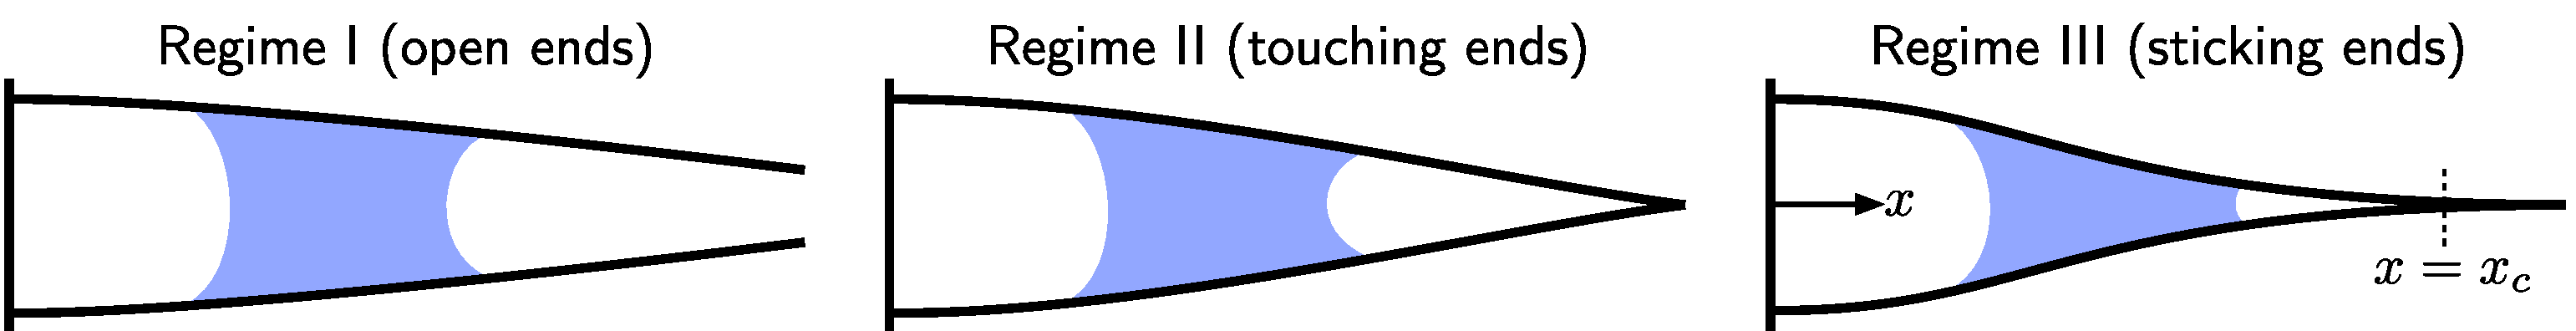
\includegraphics[width = \textwidth]{regime_schematics}
\caption{Schematic diagrams of the possible configurations of a droplet in a deformable channel that is clamped at one end: (a) open ends, (b) touching ends, and (c) sticking ends. We refer to these configurations as regime I, II and III, respectively. }\label{fig:Ch4:Geometric:RegimeSchematics}
\end{figure}

%so what happens beyond touching? introduce the idea of touching and sticking (and their names: regime II and regime III)
There are two cases for walls in contact with one another, as discussed by~\cite{Taroni2012JFM} for the case of an immobile droplet that remains in contact with the clamped end. In the first case, the channel walls make contact at a single point (they `touch', as we encountered in \S2.2). Following~\cite{Taroni2012JFM}, we refer to a channel with touching walls as being in regime II. The second case occurs when surface tension is very strong, causing the slope of the walls at the contact point to reach zero. The channel walls will make contact over a portion of their length (or `stick' together); we refer to channels with sticking walls as being in regime III. Channels whose walls are not in contact (they are `open') are referred to as being in regime I. The different possible configurations are illustrated in Figure~\ref{fig:Ch4:Geometric:RegimeSchematics}.

The model developed in Chapter 2 assumed that channels remain in regime I; to allow us to consider regimes II and III, we allow boundary conditions imposed on the channel shape at the non-clamped end (previously referred to as the free end) to change dynamically. Recall that while the channel remains in regime I, the ends are free and the appropriate boundary conditions are
\abeqn{E:Ch4:Geometric:Model:Regime1_bc}{
\ddp{^3 h}{x^3} = 0, \quad  \ddp{^2 h}{x^2} =0 \quad \text{at}~x = 1. }
Regime I applies while the channel walls remain open, i.e.
\begin{equation}\label{E:Ch4:Geometric:Model:Regime1_necessary_conditions}
h(x = 1,t) > 0.
\end{equation}
Note that our choice of an undeformed initial condition, $h(x,t = 0) = 1$, means that the channel necessarily begins in regime I.

If the walls touch during the motion, so that $h(x =1,t) = 0$ at some point, the channel enters regime II; the channel walls are no longer free at $x = 1$, but exert an equal and opposite reaction force on one another to prevent inter-penetration. We therefore replace the shear free condition~\eqref{E:Ch4:Geometric:Model:Regime1_bc}a by a contact condition. The zero moment boundary condition~\eqref{E:Ch4:Geometric:Model:Regime1_bc}b still applies; the boundary conditions imposed on channels in regime II are
\abeqn{E:Ch4:Geometric:Model:Regime2_bc}{
h = 0, \quad  \ddp{^2 h}{x^2} =0 \quad \text{at}~x = 1. }

The channel remains in regime II provided that the reaction force is repulsive (corresponding to a positive shear force), and that the slope at the contact point remains negative,
\abeqn{E:Ch4:Geometric:Model:Regime2_necessary_conditions}
{\left.\ddp{^3 h}{x^3}\right|_{x = 1} > 0, \quad \left.\ddp{h}{x}\right|_{x = 1} < 0.}
If the repulsive shear condition~\eqref{E:Ch4:Geometric:Model:Regime2_necessary_conditions}a is violated, the channel walls must open, and we return to regime I boundary conditions~\eqref{E:Ch4:Geometric:Model:Regime1_bc} (while we allow for this possibility in our numerics, we have never observed it).

If the negative slope condition~\eqref{E:Ch4:Geometric:Model:Regime2_necessary_conditions}b is violated, then the walls come into contact over a portion of their length, $x_c < x <  1$ (see Figure~\ref{fig:Ch4:Geometric:RegimeSchematics}), where $x_c > \xright$ is the location of the (a priori unknown) first point of contact between the channel walls. (We refer to this case as sticking ends since the walls appear stuck in portion $x_c <x <1$, though we emphasize that there is no adhesive force between them.) In this case, we impose smooth contact conditions at the contact point:
\abceqn{E:Ch4:Geometric:Model:Regime3_bc}{
h = 0, \quad \ddp{h}{x} = 0, \quad \ddp{^2 h}{x^2} = 0 \qquad \text{at}~x = x_c.}
and enforce a flat contact over the section of the channel walls in contact,
\begin{equation}
h = 0, \quad \ddp{h}{x} = 0 \qquad\text{for}~x_c < x < 1.
\end{equation}
Note that~\eqref{E:Ch4:Geometric:Model:Regime3_bc}c imposes an adhesion free contact between the beams~\citep{Kim2006JFM, Majidi2007MechRes} and that this additional boundary condition is necessary to determine the contact point $x_c$ as part of the solution. Channels remain in regime III while the contact point is between the `$+$' meniscus and the wall end,
\begin{equation}
\xright < x_c < 1.
\end{equation}
If $\xright$ reaches $x_c$  our model is no longer valid. If $x_c$ increases to beyond $x = 1$, the channel returns to regime II (again, this transition is allowed for in our numerics, but has not been observed).

The PDE~\eqref{E:Chapter2:Model:NonDim:CombinedEq1}--\eqref{E:Chapter2:Model:NonDim:CombinedEq3} describing the channel width,
\begin{align}
0 &= \ddp{^4 h}{x^4} & &0 < x < \xleft,\label{E:Ch4:Geometric:Model:flow_eq1}\\
\ddp{h}{t} &= \frac{1}{3|\nu|}\ddp{}{x}\left(h^3 \ddp{^5 h}{x^5}\right) & &\xleft < x <\xright, \\
0 &= \ddp{^4 h}{x^4} & &\xright < x < 1,\label{E:Ch4:Geometric:Model:flow_eq3}
\end{align}
still applies, as do the kinematic conditions~\eqref{E:Chapter2:Model:NonDim:Kinematic},
\begin{equation}\label{E:Ch4:Geometric:Model:kinematic}
\dd{x_{\pm}}{t} = -\left.\frac{h^2}{3|\nu|}\ddp{^5 h}{x^5}\right|_{x = x_{\pm}}.
\end{equation}
The boundary conditions at $x = 0$ and $x = x_{\pm}$ are as in Chapter 2 (\eqref{E:Chapter2:Model:NonDim:BCClamped}, \eqref{E:Chapter2:Model:NonDim:BCContinuity}, and~\eqref{E:Chapter2:Model:NonDim:BCPressure}); the complete set of boundary conditions for~\eqref{E:Ch4:Geometric:Model:flow_eq1}--\eqref{E:Ch4:Geometric:Model:flow_eq3} are summarised in Table~\ref{T:Ch4:Geometric:BoundaryConditions}.

\begin{table}[t!]
 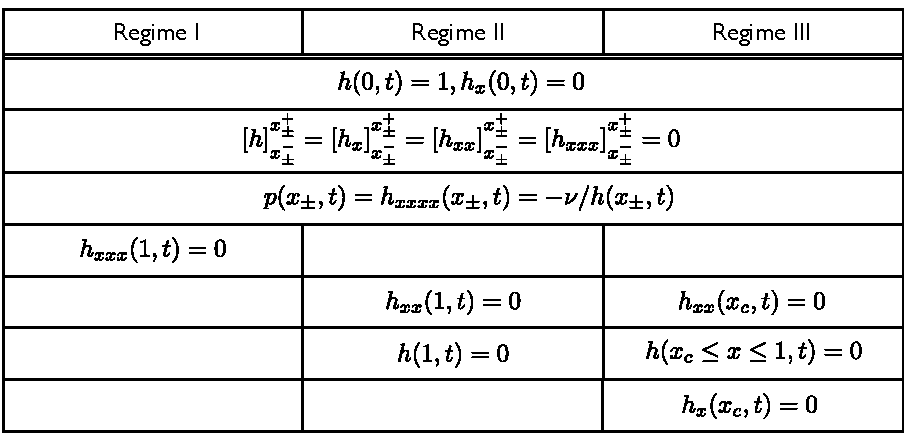
\includegraphics[scale = 0.99]{table_of_bc}
   \caption{Boundary conditions on the PDE~\eqref{E:Ch4:Geometric:Model:flow_eq1}--\eqref{E:Ch4:Geometric:Model:flow_eq3} that describes the coupled channel deflection and droplet motion in a flexible channel with either open ends (regime I), touching ends (regime II), or sticking ends (regime III). Note that subscript $x$ denotes a partial derivative in this table.}  \label{T:Ch4:Geometric:BoundaryConditions}
\end{table}

Also as in Chapter 2, we use the initial conditions
\begin{equation}\label{E:Ch4:Geometric:Model:IC}
h(x, 0) = 1,\quad \xright(0) = \xright^0, \quad \xleft(0) =\xleft^0 =  \xright^0 - V,
\end{equation}
ensuring that the dimensionless droplet volume is $V$. We note that equilibria are not possible in any of regimes I--III, because an equilibrium would require an equal channel width at both sides of the droplet.

\subsection{Numerical solutions}
To illustrate the numerical solution of the model equations (equations~\eqref{E:Ch4:Geometric:Model:flow_eq1}--\eqref{E:Ch4:Geometric:Model:IC} alongside the appropriate choice of~\eqref{E:Ch4:Geometric:Model:Regime1_bc},~\eqref{E:Ch4:Geometric:Model:Regime2_bc}, or~\eqref{E:Ch4:Geometric:Model:Regime3_bc}) we consider the cases of $\nu = 30$ and $\nu = 100$ (with $V = 0.3$, $\xright^0 = 0.4$ in each case). We shall see that with $\nu  = 30$, the simulation reaches regime II but not regime III and the simulation with $\nu = 100$ terminates while the channel is in regime III.

\subsubsection{Modifications to numerical scheme}\label{S:Geometry:Numerics}
Before presenting the dynamics of the numerical solutions, we briefly discuss the two modifications that must be made to the numerical scheme described in \S2.2.1 to implement regime II and III boundary conditions~\eqref{E:Ch4:Geometric:Model:Regime2_bc} and~\eqref{E:Ch4:Geometric:Model:Regime3_bc}, as well as dynamic changes between regimes.

\paragraph{Modification 1: isolating the drop region.}  Recall that the first step in the numerical scheme is to express the shape of the channel in the dry regions $0 < x <\xleft$ and $\xright < x < 1$ in terms of the channel shape in the drop region $\xleft < x < \xright$.  For the region $0 < x <\xleft$, we  solve~\eqref{E:Ch4:Geometric:Model:flow_eq1} alongside the clamped conditions~\eqref{E:Chapter2:Model:NonDim:BCClamped} and continuity conditions \eqref{E:Chapter2:Model:NonDim:BCContinuity}a,b;  imposing the other two continuity conditions, \eqref{E:Chapter2:Model:NonDim:BCContinuity}c,d, then results in the effective boundary conditions~\eqref{E:Chapter2:Numerics:SchemE:Chapter2:Reduced:EffectiveBCLower}, independently of the conditions at the non-clamped end. For the region $\xright < x < 1$, we solve~\eqref{E:Ch4:Geometric:Model:flow_eq3} alongside~\eqref{E:Chapter2:Model:NonDim:BCContinuity}a,b and the appropriate choice of~\eqref{E:Ch4:Geometric:Model:Regime1_bc},~\eqref{E:Ch4:Geometric:Model:Regime2_bc}, or~\eqref{E:Ch4:Geometric:Model:Regime3_bc}. Imposing the continuity conditions~\eqref{E:Chapter2:Model:NonDim:BCContinuity}c,d is then equivalent to imposing effective boundary conditions at $x = \xright$ that encode the effect of the adjacent dry region.

The channel shape in the dry region $\xright < x < 1$ (and thus effective boundary conditions applied at $x = \xright$ on the drop-only problem) must be adjusted to reflect the possible boundary conditions at the non-clamped end. Recall that for regime I configurations, the shape in the dry region $\xright < x < 1$ is expressed in terms of the shape in the drop region as
\begin{equation}
h(x,t) = \left.\ddp{h}{x}\right|_{x = \xright}(x - \xright) + \left.h\right|_{x = \xright} \qquad \xright < x <1,
\end{equation}
and the resulting effective boundary conditions are
\begin{equation}
\ddp{^2 h}{x^2} = 0, \quad \ddp{^3 h}{x^3} = 0 \quad \text{at}~x = \xright.
\end{equation}

In regime II, the channel shape in the dry region may be expressed in terms of the shape in the drop region as
\begin{multline}\label{E:Ch4:Geometric:Numerics:DryShapeRegimeII}
h(x,t) =\frac{1}{2}\left.\left[3 h + (1 -\xright)\ddp{h}{x}\right]\right|_{x = \xright} \left(\frac{1-x}{1-\xright}\right)-\\ \left.\frac{1}{2} \left[h + (1- \xright) \ddp{h}{x}\right]\right|_{x = \xright}\left(\frac{1-x}{1-\xright}\right)^3 \qquad \xright < x < 1.
\end{multline}
The resulting effective boundary conditions are
\begin{equation}
\ddp{^2 h}{x^2} = \frac{-3}{(1 - \xright)^2}\left[h + (1-\xright) \ddp{h}{x}\right],\quad \ddp{^3 h}{x^3}  =  \frac{3}{(1-\xright)^3}\left[h + (1-\xright) \ddp{h}{x} \right]
\end{equation}
at $x = \xright$.

For channels in regime III, the channel shape in the dry region is
\begin{equation}\label{E:Ch4:Geometric:Numerics:DryShapeRegimeIII}
h(x,t) = \left.h\right|_{x = \xright} \left(\frac{x_c - x}{x_c - \xright}\right)^3 \qquad \xright < x < x_c
\end{equation}
where
\begin{equation}
x_c = \xright - 3  \left.h\right|_{x = \xright} \left(\left.\ddp{h}{x}\right|_{x = \xright}\right)^{-1}.
\end{equation}
The effective boundary conditions are
\begin{equation}
\ddp{^2 h}{x^2} = \frac{6h}{(x_c - \xright)^2}, \quad \ddp{^3 h}{x^3}  = \frac{6h}{(x_c - \xright)^3} \quad \text{at}~x = \xright.
\end{equation}

\begin{figure}[t]
\centering
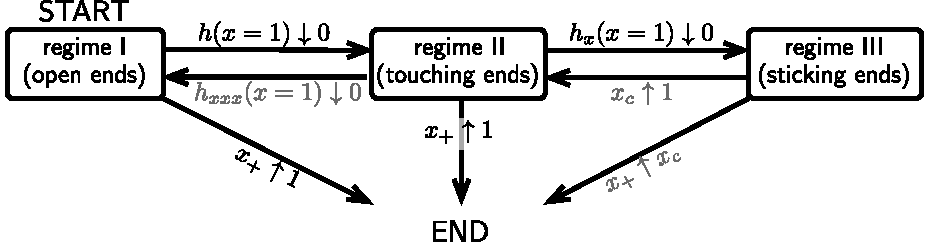
\includegraphics[scale=0.9]{geometric_numerics_events}
\caption{Flowchart of the dynamic events that trigger either a change in boundary conditions or the termination of the integration in numerical solutions of the model equations. The arrow labels indicate the event function that triggers the associated regime change or ends the simulation, and up (down) arrows indicate that the function must increase (decrease, respectively) through the value. Grey labels indicate those events that are included in the model, but are never triggered.}\label{fig:Ch4:Geometric:Flowchart}
\end{figure}

\paragraph{Modification 2: dynamically adjusting the boundary conditions.} The second  modification to the numerical scheme described in \S2.2.1 is to allow the effective boundary conditions to change dynamically. At each time-step, we determine whether changes in the boundary conditions applied at $x = x_{\pm}$ are needed, or whether the numerical integration should terminate, by evaluating event functions that indicate these transitions. These event functions, and the transitions that they trigger, are summarized in Figure~\ref{fig:Ch4:Geometric:Flowchart}. Note that in practice, we terminate the integration when the appropriate event function ($1 - \xright$ for channels in regime II, and $x_c - \xright $ for channels in regime III) comes within some tolerance of zero (we use a tolerance of $10^{-3}$ in the simulations presented here); by terminating the simulations `early', we avoid a singularity in the droplet pressure as the `$+$' meniscus advances into a channel with vanishing thickness.


\subsubsection{Dynamics}
\begin{figure}[h!]
\centering
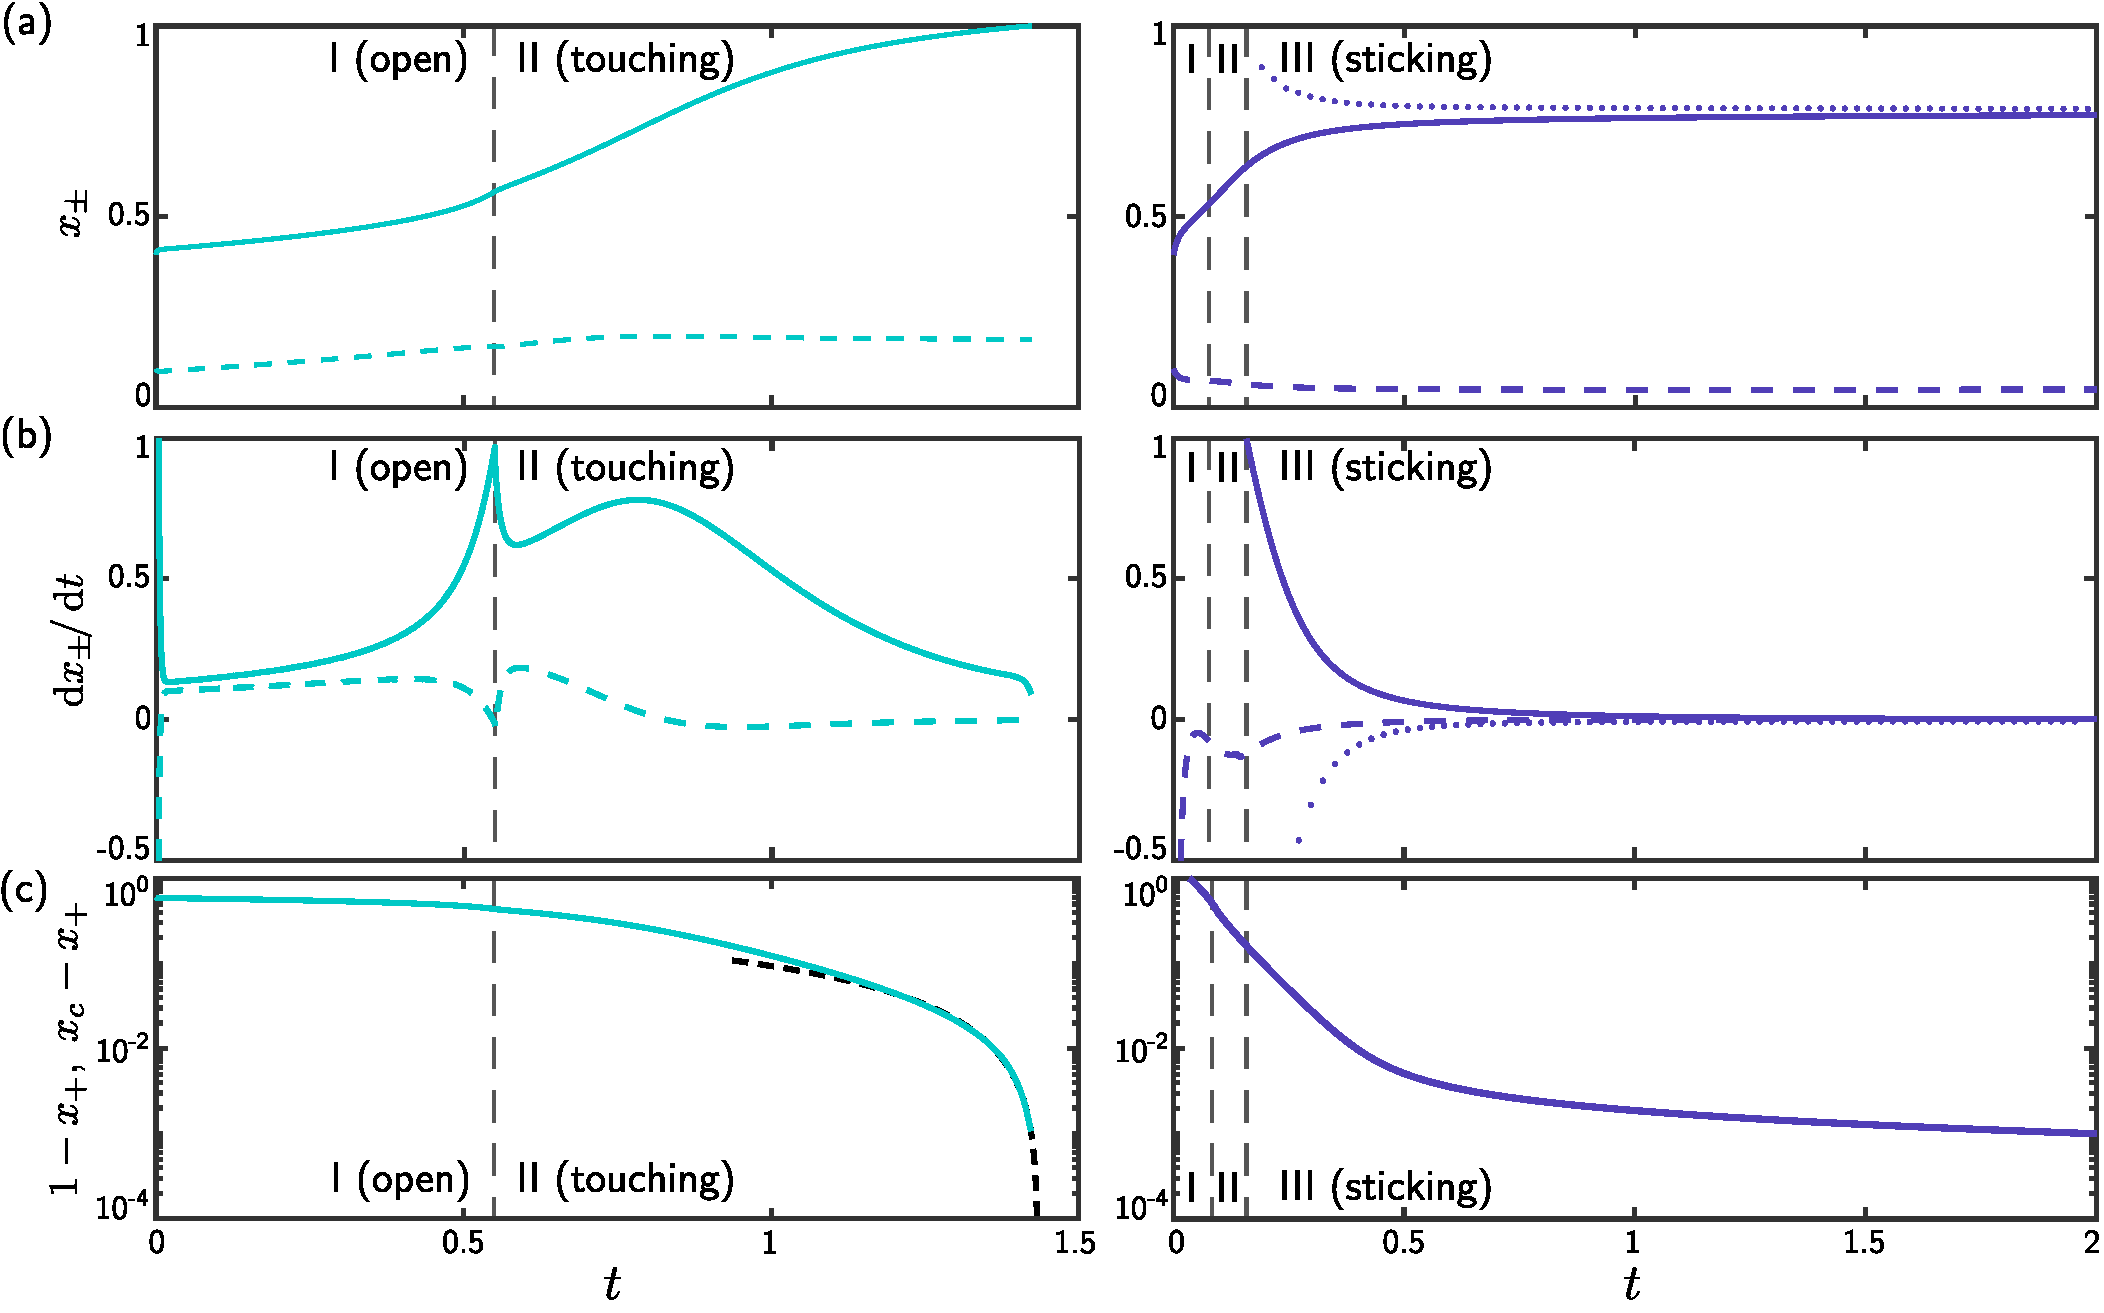
\includegraphics[width=\textwidth]{touching_and_sticking_traces}
\caption{Numerical solutions in which the system is allowed to change regimes. (a) Meniscus trajectories and (b) meniscus velocities obtained by numerically solving the model equations for $\nu = 30$ (left) and $\nu  = 100$ (right) (both solutions have $\xright^0 = 0.4$, $V = 0.3$ and use $200$ grid points). Solid and dashed curves indicate the `$+$' and `$-$' menisci, respectively; where applicable, dotted curves indicate the contact point $x_c$. (c) Plot of distance of the meniscus to the channel closure: for regimes I and II configurations (left) this is $1 - \xright$, for regime III configurations, this is $x_c - \xright$. The black dashed curve indicates the fit~\eqref{E:Ch4:Geometric:numerics:contact_time}. Vertical dashed lines indicate transitions between the various contacting conditions.}\label{fig:Ch4:geometric:numerics}
\end{figure}

Examples of the dynamic behaviour determined from the numerical solution of the model equations (allowing for changes between regimes I-III) are shown in Figure~\ref{fig:Ch4:geometric:numerics}. The left panel of Figure~\ref{fig:Ch4:geometric:numerics} shows a scenario in which the system transitions from regime I to II but appears to remain in II as $\xright \to 1$ (i.e. it does not transition to regime III). In this case, the movement of the droplet in regime I (prior to walls contacting) is dominated by translating rather than spreading -- the menisci both move in the same direction. Immediately prior to contact there is a brief spreading phase in which the leading meniscus accelerate and the rear meniscus retreats ($\mathrm{d}\xleft/\mathrm{d}t < 0$). This is reversed immediately after the contact followed by a phase in which the leading meniscus moves (at a decelerating rate) towards the contact point while the rear meniscus is approximately stationary.

By comparison, the dynamics of a system that reaches regime III are relatively simple (see right panels of Figure~\ref{fig:Ch4:geometric:numerics}).   The channel is in both regime I and II for a relatively short period of time. Throughout the motion, the `$+$' meniscus is decelerating from the high initial velocity that is a consequence of the strong early squeezing. The majority of the time is spent with the channel in regime III and $\xright$ close to $x_c$.

\subsubsection{Contact time}
%adjust discussion in previous section so we jsut say 'terminates with 1-xu = 1e-3 or xc - xu = 1e-3' discuss what happens beyond this point.
Both the simulation with $\nu = 30$  and that with $\nu = 100$ terminate when the meniscus gets within the tolerance ($10^{-3}$) of the channel end. Even with this caveat,  the curvature of the traces of $1 - \xright$ and $x_c - \xright$, shown in Figure~\ref{fig:Ch4:geometric:numerics}(c), suggest that the the meniscus would reach the channel end in finite time in the regime II case ($\nu = 30$) but would not in the regime III case ($\nu = 100$).

We have not been able to rationalize the observations using an analysis of the governing PDE. However, we note that a power law fit of the regime II case suggests that
\begin{equation}\label{E:Ch4:Geometric:numerics:contact_time}
1 - \xright \sim (t_c - t)^{5/4} \quad \text{as}~t_c - t \to 0,
\end{equation}
where $t = t_c$ is the time at which the meniscus reaches the channel end.

It is interesting to compare these results with imbibition in a rigid channel. \cite{Gorce2016Langmuir} showed that the meniscus of a column of liquid imbibing into a tapered channel with a linear profile reaches the taper `corner' linearly in time with $1 - \xright \sim t_c - t$ as $ t_c - t \to 0$ (the same imbibition behaviour was also observed for droplets by~\cite{Reyssat2014JFM}). In the present (deformable) case, the channel has a locally linear profile at the contact point ($x = 1$) when in regime II (see equation~\eqref{E:Ch4:Geometric:Numerics:DryShapeRegimeII}) and appears to make contact in finite time at a faster rate than in the rigid case ($(t_c - t)^{5/4}$ versus $(t_c - t)^1$). We believe that this is because the angle of the tapering in the flexible case may change during the motion.

\cite{Gorce2016Langmuir} also showed that  the meniscus of a column of liquid approaches the tip of a channel with a cubic profile only algebraically slowly, which appears to be in accord with the flexible case here (channels in regime III have a cubic profile near the contact point $x = x_c$, see equation~\eqref{E:Ch4:Geometric:Numerics:DryShapeRegimeIII})


\section{Trapping with hysteresis}
%
\newcommand{\hyspar}{\lambda}
\newcommand{\hysparmax}{\hyspar_{\text{max}} }
\newcommand{\hyspare}{\lambda_e}
\newcommand{\hyspari}{\lambda_{\infty}}
\newcommand{\xlefteq}{X_{-}}
\newcommand{\xrighteq}{X_{+}}
\newcommand{\xceq}{X_{c}} %meniscus poositions in equilibrium
\newcommand{\xpmeq}{X_{\pm}} %collective term for meniscus positions in equilibrium

%in reality non-unique angles
In our modelling so far, we have assumed that the contact angle between the liquid and the channel walls takes the equilibrium, or Young, value $\theta_e$ at both menisci. In reality, the contact angles are non-unique~\citep{deGennes2004}: the contact angle $\theta$ can take any value in the interval $[\theta_r, \theta_a]$ where $\theta_a$ is referred to as the advancing contact angle and $\theta_r$ is referred to as is the receding contact angle.

%what do contact angles look like in practice
A complete description of contact angle hysteresis is beyond the scope of this thesis. In this chapter, we add a simple encoding of contact angle hysteresis to the model developed in Chapter 2 and Section 4.1, which aims to capture the essential behaviour, as described by~\cite{deGennes2004}:
\begin{quote}
If, for instance, we inflate a drop (Figure~\ref{fig:Ch4:Hysteresis:primer}(a)), the contact angle $\theta$ can exceed $\theta_e$ without the line of contact moving at all. Eventually, $\theta$ reaches a threshold value $\theta_a$ beyond which the line of contact finally does move. $\theta_a$ is referred to as the advancing angle.

Likewise, when deflating a drop (Figure~\ref{fig:Ch4:Hysteresis:primer}(a)) $\theta$ can decrease down to a limiting value $\theta_r$, known as the receding angle. When $\theta = \theta_r$, the line of contact suddenly shifts.
\end{quote}
In this Chapter we supplement this static picture with the simplest possible dynamics: $\theta = \theta_a$ if the contact line is advancing and $\theta  = \theta_r$ if the contact line is receding.

Generally, contact angle hysteresis impedes droplet motion. For example, it is contact angle hysteresis that opposes gravity when slugs of liquid remain stationary in vertical capillary tubes. It has also been shown~\citep{Prakash2008Science, Bush2010AdvCollIntsci} that contact angle hysteresis, when sufficiently strong, can  arrest the motion of droplets in tapered channels that were moving as a result of the channel's tapering. We might expect a similar scenario in bendotaxis, where the droplet motion itself results from the tapering of the channel (albeit one that is induced by the droplet itself, rather than externally imposed). In this section, we aim to understand whether this expectation is correct: can contact angle hysteresis prevent droplet motion by bendotaxis? If so, when does hysteresis-induced trapping occur?

\subsection{Modelling hysteresis}\label{S:Ch4:hysteresis:modelling}
\subsubsection{Preliminaries}
\begin{figure}[t]
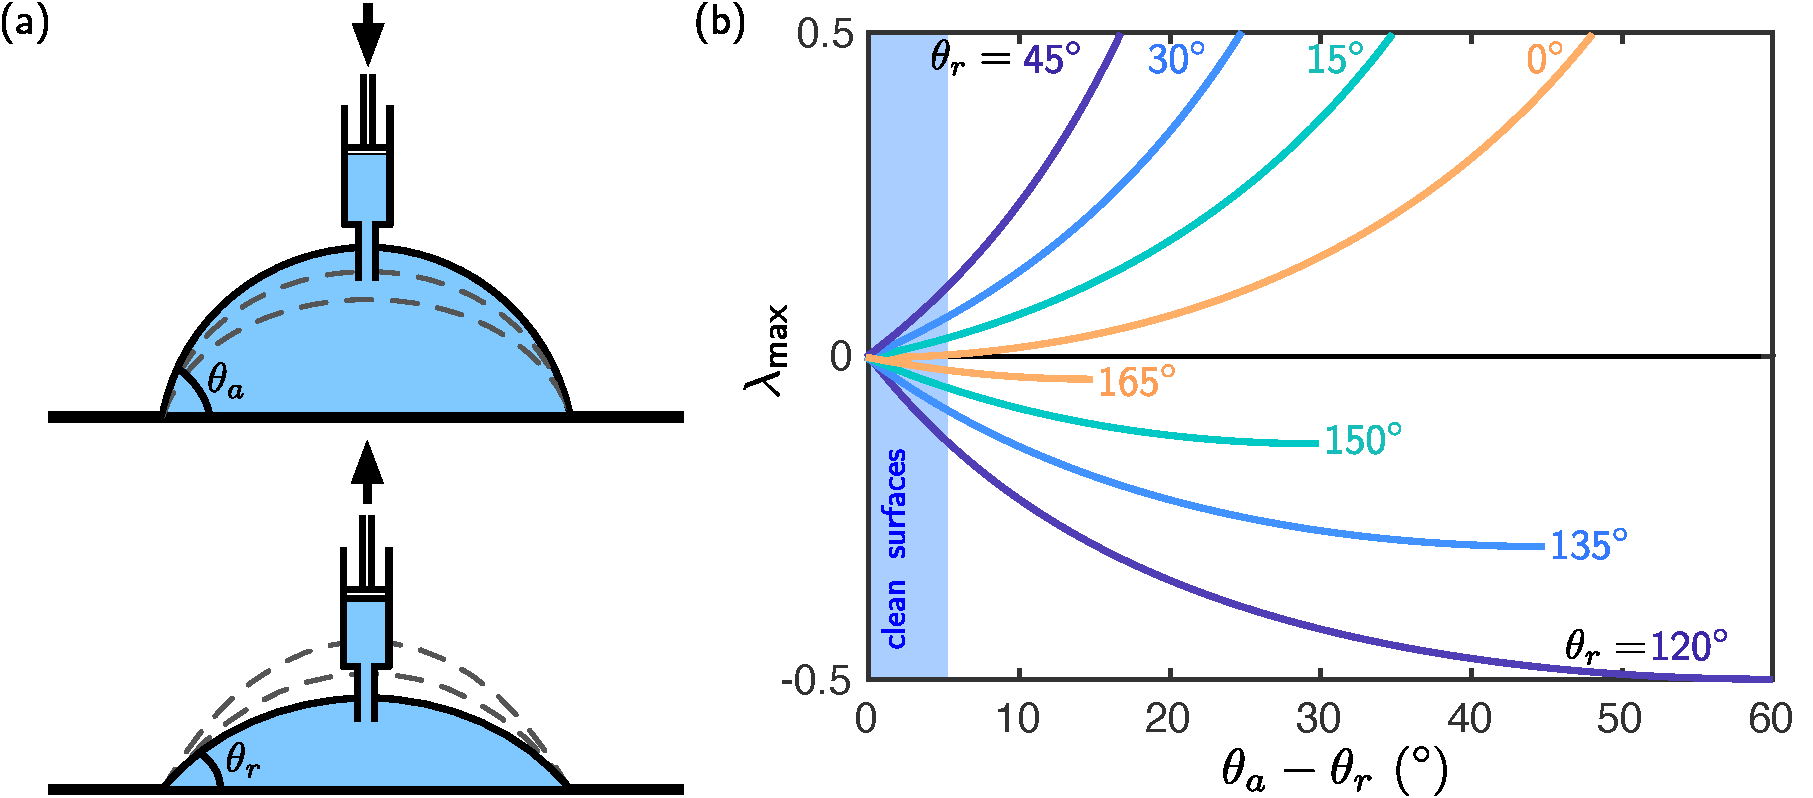
\includegraphics[scale=0.48]{cahys_primer}
\caption{(a) Schematic diagram illustrating the advancing (top) and receding (bottom) contact angles. When a droplet is being quasi-statically inflated the meniscus evolves through increasing contact angles $\theta < \theta_a$ without the contact line moving. Once $\theta = \theta_a$ the contact line advances. Similarly, when a droplet is being quasi-statically deflated, the meniscus evolves through decreasing contact angles $\theta > \theta_r$. Once $\theta = \theta_r$ the contact line recedes. (b) Plot of $\hyspar_{\text{max}}$ (equation~\eqref{E:ch4:Hysteresis:Parametrisation:hyspar_def}) as a function of $\theta_a - \theta_r$ for various receding angles $\theta_r$.  }\label{fig:Ch4:Hysteresis:primer}
\end{figure}

We present a model of contact angle hysteresis that captures the characteristic features of contact angle hysteresis described in the previous section: (i) the droplet-channel system has intrinsic advancing and receding contact angles, $\theta_a$ and $\theta_r$, respectively, with $\theta_a \geq \theta_r$, (ii) an interface is advancing (receding) if and only if the contact angle at the interface is $\theta_a$ ($\theta_r$, respectively) and (iii) the contact angle at a stationary interface may take any contact angle $\theta_r < \theta < \theta_a$.

In our system, the contact angle $\theta$ does not arise alone but rather its cosine does. It is therefore helpful to introduce the parameter
\begin{equation}\label{E:ch4:Hysteresis:Parametrisation:hyspar_def}
\hysparmax = \frac{\cos \theta_r}{\cos \theta_a} - 1
\end{equation}
as a measure of the asymmetry between the advancing and receding angles, or contact angle hysteresis. Assuming that the advancing and receding contact angles lie on the same side of 90$\si{\degree}$ (they correspond to the same wettability), then $\hysparmax >0$ for wetting configurations ($\theta_a < 90\si{\degree}$) and $\hysparmax <0$ for non-wetting configurations ($\theta_a > 90\si{\degree}$).

While this is different from the usual definition of contact angle hysteresis, $\theta_a - \theta_r$, these two measures of hysteresis are closely related:  Figure~\ref{fig:Ch4:Hysteresis:primer}(b) shows that $\hysparmax$ is monotonic in $\theta_a - \theta_r$ (increasing for wetting configurations and decreasing for non-wetting configurations). Increases in $|\hysparmax|$ therefore correspond to increases in $\theta_a - \theta_r$, and, also, $\hyspar_{\text{max}} = 0$ if and only if $\theta_a - \theta_r = 0$ (see Figure~\ref{fig:Ch4:Hysteresis:primer}(b)). Moreover,~\cite{deGennes2004} suggests that surfaces with $\theta_a - \theta_r < 5\si{\degree}$ are relatively clean (shaded in Figure~\ref{fig:Ch4:Hysteresis:primer}(b)); here $|\hysparmax|\ll 1$.

Since the contact angles at the menisci, $\theta_{\pm}(t)$, are now time-dependent, we also define
\begin{equation}\label{E:ch4:Hysteresis:Parametrisation:hyspar_dynamic_def}
\hyspar(t) =  \frac{\cos \theta_-(t)}{\cos \theta_+(t)} - 1,
\end{equation}
as measure of the instantaneous contact angle asymmetry. Within our model, $\hyspar$ has the following properties: (i) $\hyspar \leq \hyspar_{\text{max}}$ for wetting configurations and $\hyspar \geq \hyspar_{\text{max}}$ for non-wetting configurations (we will, therefore, often refer to $\hysparmax$ as the maximum contact angle asymmetry for wetting configurations), (ii)  $\hyspar = 0$ corresponds to $\theta_+ = \theta_-$ (equal contact angles at both menisci) and (iii) $\hyspar = \hyspar_{\text{max}}$ if $\theta_+ = \theta_a$ and $\theta_- = \theta_r$ (as we expect for a droplet moving towards the free end of the channel with `$+$'  meniscus advancing and `$-$' meniscus receding).

Finally, we note that in this framework, the equilibrium contact angle $\theta_e$ is no longer a relevant parameter. We must therefore choose how to replace the factors of $\cos \theta_e$ that appeared in the non-dimensionalization of Chapter 2. In the following, we use $\cos \theta_a$ in place of $\cos \theta_e$, i.e. we let
\begin{equation}\label{E:ch4:Hysteresis:Parametrisation:modified_nu_def}
\tau_c = \frac{\mu L^2}{|\gamma \cos \theta_a|H}, \quad\text{and}\quad \nu = \frac{\gamma \cos \theta_a L^4}{BH^2},
\end{equation}
respectively.

\subsubsection{Modified boundary conditions}
Incorporating this model of contact angle hysteresis into our model simply involves modifying the boundary conditions that apply at $x =x_{\pm}$, and allowing them to change dynamically. There are three cases for each meniscus, depending on its current motion and the contact angle there. Throughout, we keep in mind that the kinematic conditions and Laplace pressure conditions, which now read
\abeqn{E:ch4:Hysteresis:Parametrisation:kbc_and_laplace}{
\dd{x_{\pm}}{t} = \left. \frac{-h^2}{3|\nu|}\ddp{^5 h}{x^5}\right|_{x = x_{\pm}} \quad \text{and} \quad \left.\ddp{^4 h}{x^4}\right|_{x =x_{\pm}} = -\frac{\nu}{h(\xright,t)}\frac{\cos \theta_{\pm}}{\cos \theta_a},}
respectively, always hold.

Consider first the `$+$' meniscus. If this is moving with a positive velocity (corresponding to a negative pressure gradient), it is advancing out of the liquid so $\theta_+ = \theta_a$, i.e. we set
\begin{equation}\label{E:ch4:Hysteresis:Parametrisation:BC+_advancing}
\theta_+ = \theta_a, \qquad \text{if}~\dd{\xright}{t} > 0.
\end{equation}

If the `$+$' meniscus subsequently stops moving (the pressure gradient decreases to zero), it is then pinned in place; its contact angle $\theta_+$ takes the value between $\theta_r$ and $\theta_a$  (via the Laplace pressure condition~\eqref{E:ch4:Hysteresis:Parametrisation:kbc_and_laplace}b) that maintains zero pressure gradient, i.e. we set \begin{equation}\label{E:ch4:Hysteresis:Parametrisation:BC+_pinned}
\theta_r \leq \theta_+ \leq \theta_a \quad \text{if}~\dd{\xright}{t}  = 0.
\end{equation}
Should the contact angle increase back up to $\theta_a$ while the meniscus is pinned, we return to the advancing conditions~\eqref{E:ch4:Hysteresis:Parametrisation:BC+_advancing}. If, on other hand, the contact angle decreases down to $\theta_r$, the meniscus begins to recede into the liquid (it moves with a negative velocity) taking the receding angle, i.e. we set
\begin{equation}\label{E:ch4:Hysteresis:Parametrisation:BC+_receding}
\theta_+ = \theta_r \qquad \text{if}~\dd{\xright}{t} <0.
\end{equation}
The transition from receding back to pinned occurs if the meniscus velocity increases back to zero from below.

The conditions on $\theta_-$ are very similar: precisely one of
\renewcommand*{\arraystretch}{1.3}
\abceqn{E:ch4:Hysteresis:Parametrisation:BC_xleft}{
\left\{
\begin{matrix}
\theta_- = \theta_a & \dd{\xleft}{t} < 0,\\
\theta_r < \theta_- < \theta_a  &\dd{\xleft}{t} =  0,\\
\theta_- = \theta_r & \dd{\xleft}{t} > 0,
\end{matrix} \right.}
must hold at all times. (The small differences between the contact angle conditions on $\theta_+$ and $\theta_-$ are a result of being located on opposite sides of the droplet, so that advancing and receding have opposing senses for the two menisci.)

To close the model, we need to specify initial conditions on the contact angles $\theta_\pm$. To be consistent with the early squeezing, in which the menisci move in opposite directions (away one another for wetting configurations, and towards from one another for non-wetting configurations), we take initial conditions
\begin{equation}\label{E:ch4:Hysteresis:Parametrisation:ic_theta_wetting}
\theta_{\pm}(t = 0) = \theta_a
\end{equation}
for wetting conditions (i.e. if $\hyspar > 0, \nu >0$) and
\begin{equation}
\theta_{\pm}(t = 0) = \theta_r
\end{equation}
for non-wetting conditions ($\hyspar < 0, \nu <0$). Here, we shall focus primarily on wetting conditions, which display more diverse behaviour (the different contacting regimes discussed in \S\ref{S:Ch4:Geometric} are only possible for wetting conditions); we discuss the corresponding results for non-wetting configurations in \S\ref{S:Ch4:Hysteresis:NonWetting}.

\subsection{Numerical Solutions}\label{S:Ch4:Hysteresis:Numerics}

\begin{figure}[t]
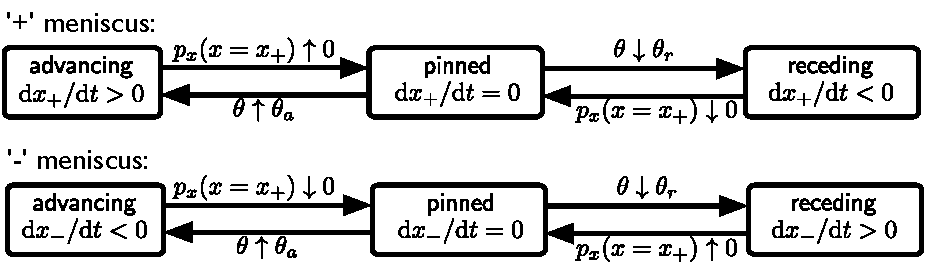
\includegraphics[scale = 0.97]{transitions_contact_angles}
\caption{Flowchart of the dynamic events that result in a change of boundary conditions in the model equations describing bendotaxis with contact angle hysteresis. The arrow labels indicate the function that triggers the transition, and up (down) arrows indicate that the function must increase (decrease, respectively) through the corresponding value.}\label{fig:Ch4:Hysteresis:Flowchart}
\end{figure}

\begin{figure}[h!]
\centering
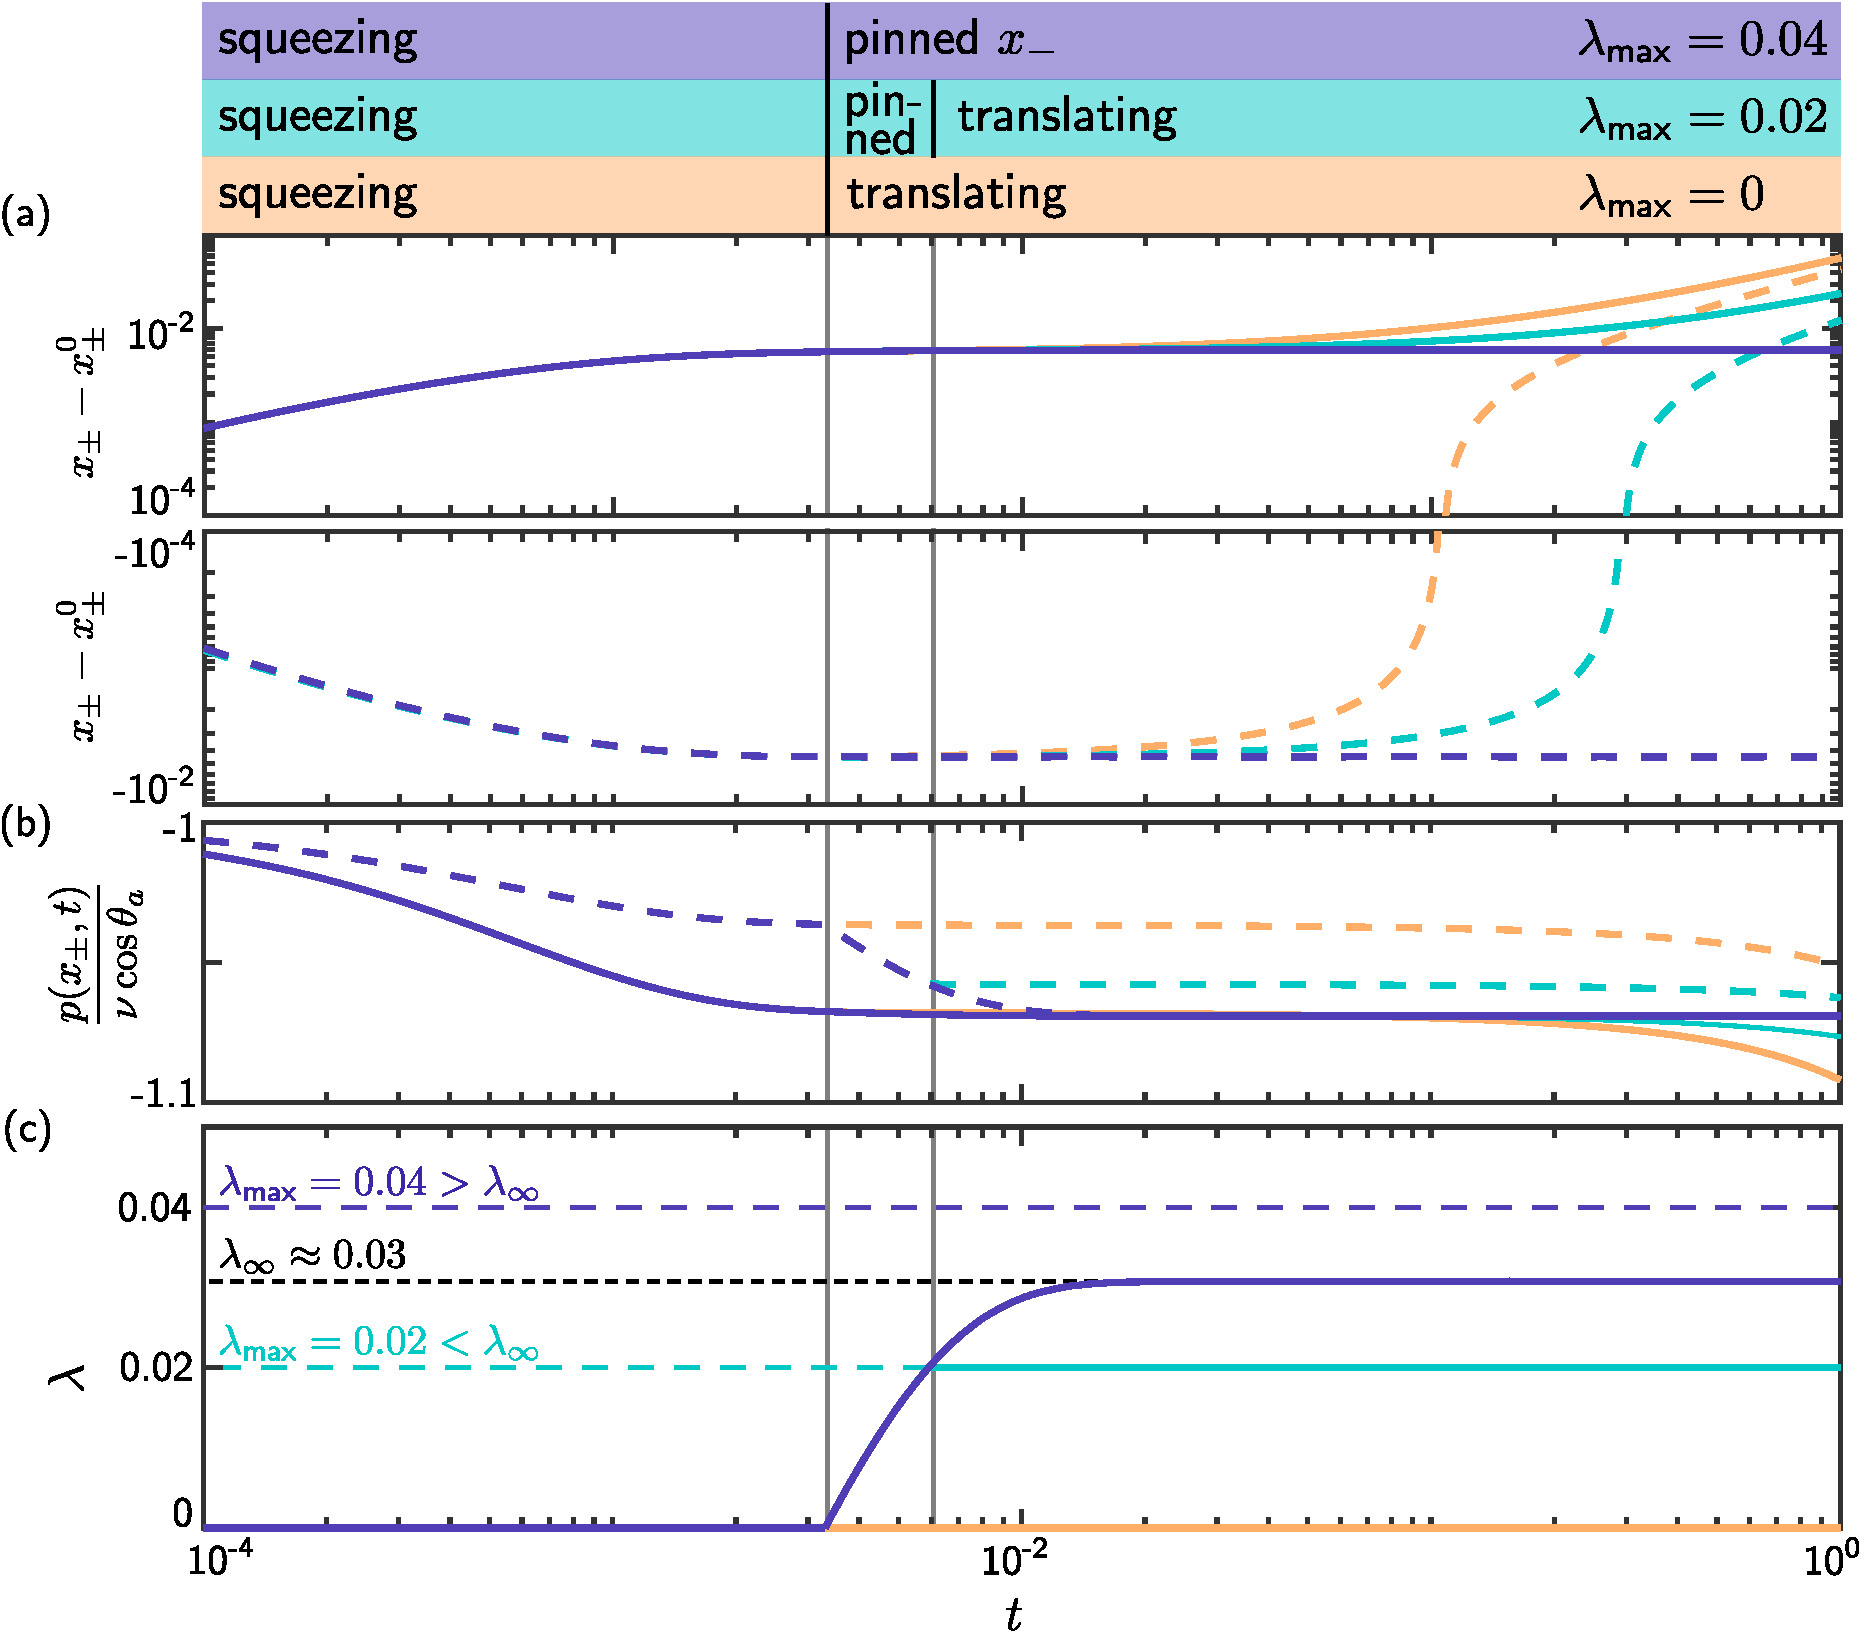
\includegraphics[width = 0.9\textwidth]{example_solutions_stacked_v3}
\caption{Numerical simulations of bendotaxis with contact angle hysteresis. The plots show (a) the displacement of the menisci away from their initial positions, (b) the normalized meniscus pressure, and (c) the contact angle asymmetry $\hyspar$.  In each plot, solid curves correspond to results for the `$+$' meniscus while dashed curves correspond to  results for the `$-$' meniscus. In each case, $\theta_r = 0\si{\degree}$, and solutions are shown for three different values of the contact angle hysteresis $\hyspar_{\text{max}}$ as follows: $\hyspar_{\text{max}} = 0$ (orange curves, i.e.~no contact angle hysteresis), $\hyspar_{\text{max}} = 0.02$ (green curves,  $\theta_a = 10\si{\degree}$ -- relatively small contact angle hysteresis), and $\hyspar_{\text{max}} = 0.04$ (purple curves, $\theta_a = 16\si{\degree}$ -- relatively large contact angle hysteresis). In each case, $\nu =  4, \xright^0 = 0.65, V = 0.2$ (i.e. $\xleft^0= 0.45$).  A log-log scale is used in (a) to aid distinction between the curves. The motion can be split into (at most) three temporal regions based on the direction of motion of the menisci; these are referred to as squeezing, pinned $\xleft$, and translating as indicated at the top of the figure. In (c), the coloured horizontal dashed lines indicate the corresponding value of $\hyspar = \hysparmax$ and the black dashed line indicates $\hyspar = \hyspar_{\infty}$ -- the contact angle asymmetry that the system would saturate at for $\hyspar_{\text{max}} \gg 1$ (see main text).}\label{fig:Ch4:Hysteresis:ExampleTraces}
\end{figure}


In this section, we consider numerical solutions of the system~\eqref{E:Ch4:Geometric:Model:flow_eq1}--\eqref{E:Ch4:Geometric:Model:flow_eq3} with the boundary conditions listed in Table~\ref{T:Ch4:Geometric:BoundaryConditions} and modified kinematic conditions~\eqref{E:ch4:Hysteresis:Parametrisation:kbc_and_laplace}--\eqref{E:ch4:Hysteresis:Parametrisation:ic_theta_wetting}. These numerical solutions offer insight into how hysteresis affects the dynamics of bendotaxis, showing how the various transitions between boundary conditions described in \S\ref{S:Ch4:hysteresis:modelling} might occur in practice, and offer insight into one route by which droplets may be trapped within a channel.

\subsubsection{Modifications to numerical scheme}
It is straightforward to modify the numerical scheme described in \S2.2 and \S4.1.2 to include contact angles that evolve dynamically within this model of hysteresis. Transitions between advancing, pinned, and receding conditions at each meniscus are determined by evaluating appropriate event-detection functions at each time-step, as outlined in the flowchart in Figure~\ref{fig:Ch4:Hysteresis:Flowchart}. Note that several of the nine possible (three at each meniscus) combinations of states (advancing, pinned or receding) for $(\theta_+, \theta_-)$ are not realizable as they would require a violation of conservation of mass; for example, receding angles at both menisci, $\theta_+ = \theta_r, \theta_- = \theta_r$, is incompatible with wetting conditions in which the channel walls are deflected inwards.

Note that here we consider only channels in regime I (open ends), although our numerical scheme is capable of describing any combination of the boundary conditions at $x = x_{\pm}$ and $x = 1$ that arise from the various contact angle and contacting conditions described in \S4.1 and \S\ref{S:Ch4:hysteresis:modelling}.

\subsubsection{Dynamics}
In Figure~\ref{fig:Ch4:Hysteresis:ExampleTraces}, we show numerically obtained traces of the displacement of the menisci, the normalized meniscus pressure, and contact angle asymmetry for three different values the advancing contact angle as follows: $\theta_a = 0\si{\degree}$,  $\theta_a = 10\si{\degree}$, and $ \theta_a =16\si{\degree}$, all with $\theta_r = 0\si{\degree}$. The corresponding values of the contact angle hysteresis $\hysparmax$ are $\hysparmax = 0$, $\hysparmax = 0.02$, and $\hysparmax = 0.04$, respectively. (These correspond to systems with no contact angle hysteresis, relatively small contact angle hysteresis and relatively large contact angle hysteresis, respectively, as we shall see.)

\paragraph{Initial behaviour.}
The three solutions have identical initial conditions ($\xright^0 = 0.65, \xleft^0 =0.45$), and are thus identical at early times (the droplet does not have any information about the maximum possible contact angle asymmetry, $\hyspar_{\text{max}}$, while $\hyspar < \hyspar_{\text{max}}$). In this squeezing period, the droplet has the advancing contact angle at both menisci, so $\hyspar = 0$ (Figure~\ref{fig:Ch4:Hysteresis:ExampleTraces}(c)) and the behaviour is identical to the early time behaviour described in Chapter 2 -- the droplet responds to the initial torque imbalance and the pressure decreases with time at both menisci as the confinement becomes stronger (Figure~\ref{fig:Ch4:Hysteresis:ExampleTraces}(b)).

\paragraph{Pinning of $\xleft$.}
As the channel continues to deform inwards, the pressure gradient at $\xleft$ decreases, eventually reaching zero so that this meniscus becomes pinned -- the advancing boundary condition~\eqref{E:ch4:Hysteresis:Parametrisation:BC_xleft}a is replaced by the pinned boundary condition~\eqref{E:ch4:Hysteresis:Parametrisation:BC_xleft}b. We refer to the subsequent time period as `pinned $\xleft$' to reflect this change in boundary conditions (see Figure~\ref{fig:Ch4:Hysteresis:ExampleTraces}).

The behaviour of the solutions for different values of $\hyspar_{\text{max}}$ diverges at this point: if $\hyspar_{\text{max}} = 0$, the pinned meniscus  immediately unpins (since $\theta_a = \theta_r = 0\si{\degree}$ throughout). The meniscus $\xleft$ turns and moves towards the free end (orange traces in Figure~\ref{fig:Ch4:Hysteresis:ExampleTraces}); these dynamics are precisely those discussed in Chapter 2.

For $\hyspar_{\text{max}} > 0$, $\xleft$ remains pinned for a  period of time.  $\xright$ continues to advance and the channel deformation continues to increase, thus reducing the pressure at $\xright$ (increasing the suction) and maintaining $\theta_+ = \theta_a$. To maintain a pinned condition at $\xleft$, the contact angle difference $\hyspar$  increases (the contact angle $\theta_-$ decreases, increasing $\cos \theta_-$, which acts to increase the magnitude of the suction pressure via the Laplace pressure condition~\eqref{E:ch4:Hysteresis:Parametrisation:kbc_and_laplace}). Independent of the value of $\hysparmax$, there is a limit to how much the channel can deform, and thus to how much the pressure can change, while $\xleft$ remains pinned. There is therefore a value of $\hyspar$, which we denote by $\hyspari$, at which the meniscus remains pinned indefinitely and reaches equilibrium. The value of $\hyspari$ depends on $\nu, V, \xright^0$ but emerges from the dynamic model -- it is not possible to determine it a priori, though our simulations suggest $\hyspari = 0.03$ for the values $\nu = 4, V = 0.2, \xright^0 = 0.65$ used here.

Whether the droplet leaves the pinned $\xleft$ stage depends on whether $\hyspar$ reaches $\hyspari$ without first reaching the maximum allowed contact angle asymmetry $\hysparmax$, at which point $\xleft$ must de-pin. If the contact angle hysteresis is relatively large then $\hysparmax > \hyspari$ (purple curves in Figure~\ref{fig:Ch4:Hysteresis:ExampleTraces}), so $\hyspar$ reaches $\hyspari$ first, and, when it does so, the droplet remains trapped partway along the channel with $\xleft$ pinned indefinitely. If the contact angle hysteresis is relatively small, then $\hysparmax \leq \hyspari$ (green curves in Figure~\ref{fig:Ch4:Hysteresis:ExampleTraces}), so $\hyspar$ reaches the maximum allowed asymmetry, $\hysparmax$, and the $\xleft$ contact line de-pins. We therefore have $\theta_- = \theta_r$ (recall that $\theta_+ = \theta_a$ still) and the droplet begins to translate to the free end of the channel. In summary, when contact angle hysteresis is small, the maximum contact angle asymmetry $\hysparmax$ is insufficient to maintain the pinned $\xleft$ state and the droplet translates to the free end via bendotaxis. If the maximum allowed asymmetry is sufficiently large, $\hysparmax > \hyspari$, then the droplet is trapped. (Note that as $\hysparmax \to \infty$, the contact angle asymmetry will always saturate at $\hyspar = \hyspari$.)

%if we reach the third period, droplet escapes. A point to make is that this sequential behaviour is generic (i.e. wetting droplets always do period 1 -> period 2 OR period 1-> period 2 -> period 3, and we only see at most three of the possible 9 combinations of boundary conditions).


\subsubsection{Discussion of dynamics}
These numerical solutions highlight two important points: firstly, they demonstrate that even a moderate amount of hysteresis can have a significant influence on the dynamics of bendotaxis; in the  simulation with relatively small contact angle hysteresis ($\theta_a =  10\si{\degree}$, $\theta_r =  0\si{\degree}$) the droplet takes approximately twice as long to reach the free end as the case of no hysteresis ($\theta_a =  \theta_r =  0\si{\degree}$). (This sensitivity of the dynamics to contact angle hysteresis justifies the care taken to minimize it in the experimental study of bendotaxis presented in Chapter 3.)

Secondly, these simulations confirm our intuition that when hysteresis is sufficiently strong, droplets may get trapped part way along the channel. The numerical solutions highlight three important features of the trapping mechanism, that appear to be generic:
firstly, the system always passes through a squeezing period, after $\xleft$ is pinned; secondly there is a contact angle asymmetry, $\hyspari$, required to maintain the pinned conditions indefinitely; and, thirdly, if $\hysparmax \leq \hyspari$, the maximum contact angle asymmetry is not enough to pin the droplet and it begins to translate, but if $\hysparmax > \hyspari$ the droplet remains in the pinned state.

\subsubsection{Effect of droplet initial position}
\begin{figure}[t]
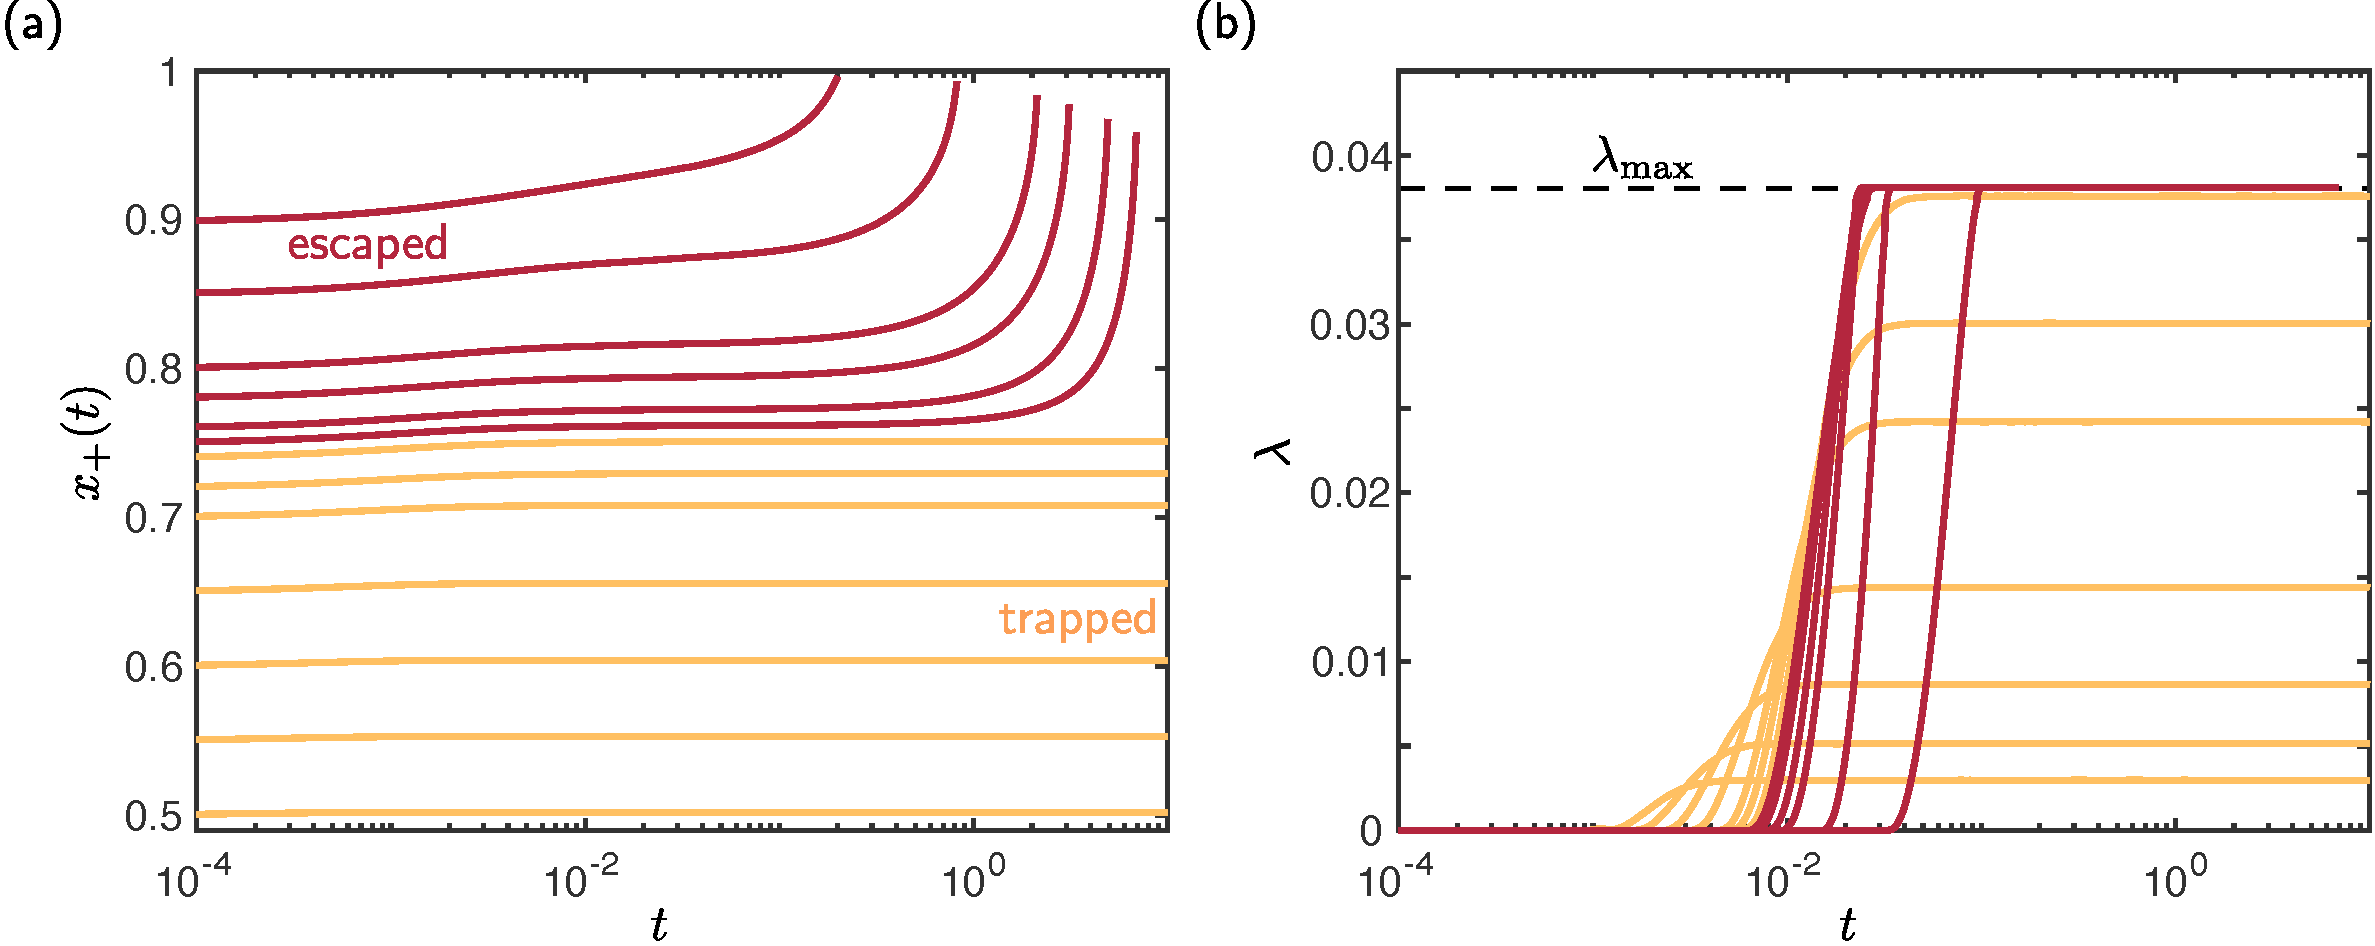
\includegraphics[width = 0.95\textwidth]{escape_traces}
\caption{(a) Meniscus position $\xright(t)$ and (b) contact angle asymmetry $\hyspar$ in simulations of bendotaxis with contact angle hysteresis
for various initial meniscus positions in the range $0.5\leq \xright^0 \leq0.9$.  For each value of $\xright^0 = \xright(t = 0)$, $V = 0.2,~ \nu = 4,~ \hyspar_{\text{max}} = 0.038, ~\theta_r = 0\si{\degree}$ (corresponding to an advancing angle $\theta_a = 18\si{\degree}$). Note that droplets starting close to the free end ($\xright^0$ sufficiently large) escape, whilst those starting closer to the base are trapped indefinitely.}\label{fig:Ch4:Hysteresis:Numerics:initialpos}
\end{figure}

Further insight into the trapping mechanism can be gleaned by considering the effect of the initial position of the `$+$' meniscus, $\xright^0$. In Figure~\ref{fig:Ch4:Hysteresis:Numerics:initialpos}, we plot numerically obtained trajectories $\xright(t)$ and the corresponding evolution of the contact angle asymmetry $\lambda(t)$ for various initial conditions in the range $0.5 \leq \xright^0 \leq 0.9$. We see that for droplets that start close to the free end, $\hyspar$ reaches $\hysparmax$ so that the droplet begins to translate and ultimately reaches the free end (it `escapes'). However, for droplets that start closer to the base (smaller values of $\xright^0$), $\hyspar$ does not reach $\hysparmax$ before $\hyspari$ and the droplet remains trapped part way along the channel, close to its initial position. This behaviour suggests that $\hyspari$ is an increasing function of $\xright^0$, as we might expect -- a greater contact angle difference will be needed to maintain the pinned state when the droplet sits nearer the free end of the channel, which is easier to deform.

In the remainder of this chapter, we address the following question that is motivated by the dynamic numerical solutions just presented: when (i.e. in which regions of $(\nu, V, \xright^0, \hysparmax)$ space) do droplets get trapped as a result of contact angle hysteresis? The first step in approaching this question is to consider the configurations occupied when droplets are trapped, i.e. equilibria of the system, and so we turn to this now.
\subsection{Equilibrium configurations}\label{S:Ch4:Hysteresis:Equilibria}
The numerical solutions presented in \S\ref{S:Ch4:Hysteresis:Numerics} suggest that droplets can be trapped indefinitely if the contact angle hysteresis is sufficiently large (or equivalently that droplets start sufficiently close to the clamped end). In this section, we consider these trapped equilibrium states. We aim to determine when equilibria exist and analyse their linear stability, with a view to (i) verifying that the numerical solutions presented in \S\ref{S:Ch4:Hysteresis:Numerics} are indeed converging to true equilibria (rather than simply slowly evolving transients), (ii) checking that these equilibria are linearly stable and (iii) understanding whether it is ever possible for a droplet to become trapped after reaching the translating phase.

In this section, we consider equilibrium configurations for a general contact angle difference $\hyspar = \hyspare$; these results are then expected to be pertinent provided that $\hyspare$ is attainable, i.e. provided that $\hyspare \leq \hysparmax$.

\subsubsection{Equations for equilibrium}
%state the equations for equilibria, and an appendix describing how we solve them numerically (but mention key point that we don't actually specify V but rather xright). In particular, point out that the hysteresis condition can be thought of as a geometric constraint.
Equilibrium configurations can be recovered from the steady form of the dynamic problem (the PDE~\eqref{E:Ch4:Geometric:Model:flow_eq1}--\eqref{E:Ch4:Geometric:Model:flow_eq3} with the boundary conditions in Table~\ref{T:Ch4:Geometric:BoundaryConditions} but with the Laplace pressure condition replaced by~\eqref{E:ch4:Hysteresis:Parametrisation:kbc_and_laplace}b). Here we consider configurations in regime I, II or III, for completeness, but we are primarily interested in regime I because droplets in channels in regime II or III are already trapped (albeit via a different mechanism). As we shall see, only regime I equilibria exist in the region of parameter space of interest.

The problem for the equilibrium channel wall shape $h_e(x)$ with menisci located at $x_{\pm} = \xpmeq$ (as well as possibly for the contact point $x_c =\xceq$) is
\begin{align}
\dd{^4 h_e}{x^4} &= 0, & &\text{for}~ 0 < x < \xlefteq,\label{E:Ch4:Hyseresis:Equilibria:Eqs:Beam1}\\
\dd{^4 h_e}{x^4} &= p_0, & &\text{for}~ \xlefteq < x < \xrighteq,\label{E:Ch4:Hyseresis:Equilibria:Eqs:Beam2}\\
\dd{^4 h_e}{x^4} &= 0, & &\text{for}~ \xrighteq < x < 1,\label{E:Ch4:Hyseresis:Equilibria:Eqs:Beam3}
\end{align}
where $p_0$ is the equilibrium droplet pressure. $p_0$ is constant throughout the droplet (since we consider equilibrium) and so, in particular, the meniscus pressures equal $p_0$, i.e.
\begin{equation}\label{E:Ch4:Hyseresis:Equilibria:Eqs:BeamP}
p_0 = -\left.\frac{\nu}{h_e}\right|_{x = \xrighteq}  = -\left.\frac{\nu(1 + \hyspare) }{h_e}\right|_{x = \xlefteq}.
\end{equation}

The problem~\eqref{E:Ch4:Hyseresis:Equilibria:Eqs:Beam1}--\eqref{E:Ch4:Hyseresis:Equilibria:Eqs:BeamP} must be solved subject to further boundary conditions
\begin{equation}\label{E:Ch4:Hyseresis:Equilibria:Eqs:ClampedBC}
h_{e} = 1,\quad  \dd{h_e}{x} = 0, \quad \text{at}~x = 0,
\end{equation}
continuity conditions
\begin{equation}\label{E:Ch4:Hyseresis:Equilibria:Eqs:Continuity}
\left[h_e\right]_{\xpmeq^-}^{\xpmeq^+} = \left[\dd{h_e}{x}\right]_{\xpmeq^-}^{\xpmeq^+} = \left[\dd{^2 h_e}{x^2}\right]_{\xpmeq^-}^{\xpmeq^+}=\left[\dd{^3 h_e}{x^3}\right]_{\xpmeq^-}^{\xpmeq^+}  =0,
\end{equation}
and boundary conditions at the non-clamped end, which depend on the regime as:
\begin{align}
\left.\dd{^2 h_e}{x^2}\right|_{x = 1}  = \left.\dd{^3 h_e}{x^3}\right|_{x = 1} &= 0   & &\text{regime I (open ends),}\label{E:Ch4:Hyseresis:Equilibria:Eqs:FarEndBCFree}\\
\left.h_e\right|_{x = 1}  =   \left.\dd{^2 h_e}{x^2}\right|_{x = 1}&= 0  & &\text{regime II (touching ends),}\label{E:Ch4:Hyseresis:Equilibria:Eqs:FarEndBCTouching}\\
h_e(\xceq \leq x \leq 1) = \left.\dd{h_e}{x}\right|_{x = \xceq} =   \left.\dd{^2 h_e}{x^2}\right|_{x =\xceq} &= 0    & &\text{regime III (sticking ends).}\label{E:Ch4:Hyseresis:Equilibria:Eqs:FarEndBCSticking}
\end{align}
The solution $h_e(x)$ must also satisfy the global volume constraint,
\begin{equation}\label{E:Ch4:Hyseresis:Equilibria:Eqs:Volume}
V = \int_{\xlefteq}^{\xrighteq}h_e(x)~\mathrm{d}x.
\end{equation}

For any candidate equilibrium, we must also ensure that
\begin{align}
&h_e(1) > 0 & &\textsf{for regime I,}\label{E:Ch4:Hyseresis:Equilibria:Eqs:regimeI_constraint}\\
&\left.\dd{^3 h_e}{x^3}\right|_{x = 1} >0, \quad \left.\dd{h_e}{x}\right|_{x =1} <0 & &\textsf{for regime II,}\label{E:Ch4:Hyseresis:Equilibria:Eqs:regimeII_constraint}\\
&\xrighteq < \xceq < 1 & &\textsf{for regime III,}\label{E:Ch4:Hyseresis:Equilibria:Eqs:regimeIII_constraint}
\end{align}
as discussed in \S\ref{S:Ch4:Geometric:Model}.

Note that by re-arranging~\eqref{E:Ch4:Hyseresis:Equilibria:Eqs:BeamP}, the contact angle asymmetry $\hyspare$ can be expressed as a geometric constraint on the solution:
\begin{equation}\label{E:Ch4:Hyseresis:Equilibria:Eqs:hyspar_geometry}
\hyspare = \frac{h_e(\xlefteq)}{h_e(\xrighteq)} - 1.
\end{equation}

\subsubsection{Equilibria with $\xlefteq = 0$}
The equations for equilibrium~\eqref{E:Ch4:Hyseresis:Equilibria:Eqs:Beam1}--\eqref{E:Ch4:Hyseresis:Equilibria:Eqs:Volume} do not have an analytic solution in general. However, analytic progress can be made if we impose (instead of solving for) $\xlefteq = 0$. Although this is case is hypothetical (we do not expect the Laplace pressure boundary condition to hold when the liquid contacts the base, for example), it serves as a limiting case and will be useful in what follows.

In this case, the combination of the pressure condition~\eqref{E:Ch4:Hyseresis:Equilibria:Eqs:BeamP} and the clamped boundary condition~\eqref{E:Ch4:Hyseresis:Equilibria:Eqs:ClampedBC} mean that equilibrium pressure is simply $p_0 = \nu (1 + \hyspare)$, and we can find  analytic solutions with channel shapes
\begin{equation}\label{E:Ch4:Hyseresis:Equilibria:Eqs:analytic_sol}
h_e(x) = 1-\frac{\nu(\hyspare +1)}{24}\times\begin{cases} (x-\xrighteq)^4 + 4\xrighteq^3(x-\xrighteq) + 3\xrighteq^4, & 0 < x < \xrighteq\\
\xrighteq^3 (4x-\xrighteq) & \xrighteq < x <1.
\end{cases}
\end{equation}
where the meniscus position $\xrighteq$ satisfies
\begin{equation}\label{E:Ch4:Hyseresis:Equilibria:Eqs:analytic_sol_meniscus_position}
\xrighteq^4 = \frac{8\hyspare}{\nu (1 + \hyspare)^2}.
\end{equation}
To satisfy the volume constraint~\eqref{E:Ch4:Hyseresis:Equilibria:Eqs:Volume} we require
\begin{equation}\label{E:Ch4:Hyseresis:Equilibria:Eqs:analytic_sol_volume}
\nu = \frac{8}{V^4}\frac{\hyspare}{(1+\hyspare)^2}\left(\frac{3\hyspare + 5}{5\hyspare + 5}\right)^4.
\end{equation}
Provided~\eqref{E:Ch4:Hyseresis:Equilibria:Eqs:analytic_sol_volume} holds, the open ends constraint~\eqref{E:Ch4:Hyseresis:Equilibria:Eqs:regimeI_constraint} is
\begin{equation}\label{E:Ch4:Hyseresis:Equilibria:Eqs:analytic_sol_open_ends}
V > \frac{4\hyspare(3\hyspare + 5)}{5(\hyspare+1)(4\hyspare + 3)}.
\end{equation}

\subsubsection{Regime Diagrams}
\begin{figure}[t]
\centering
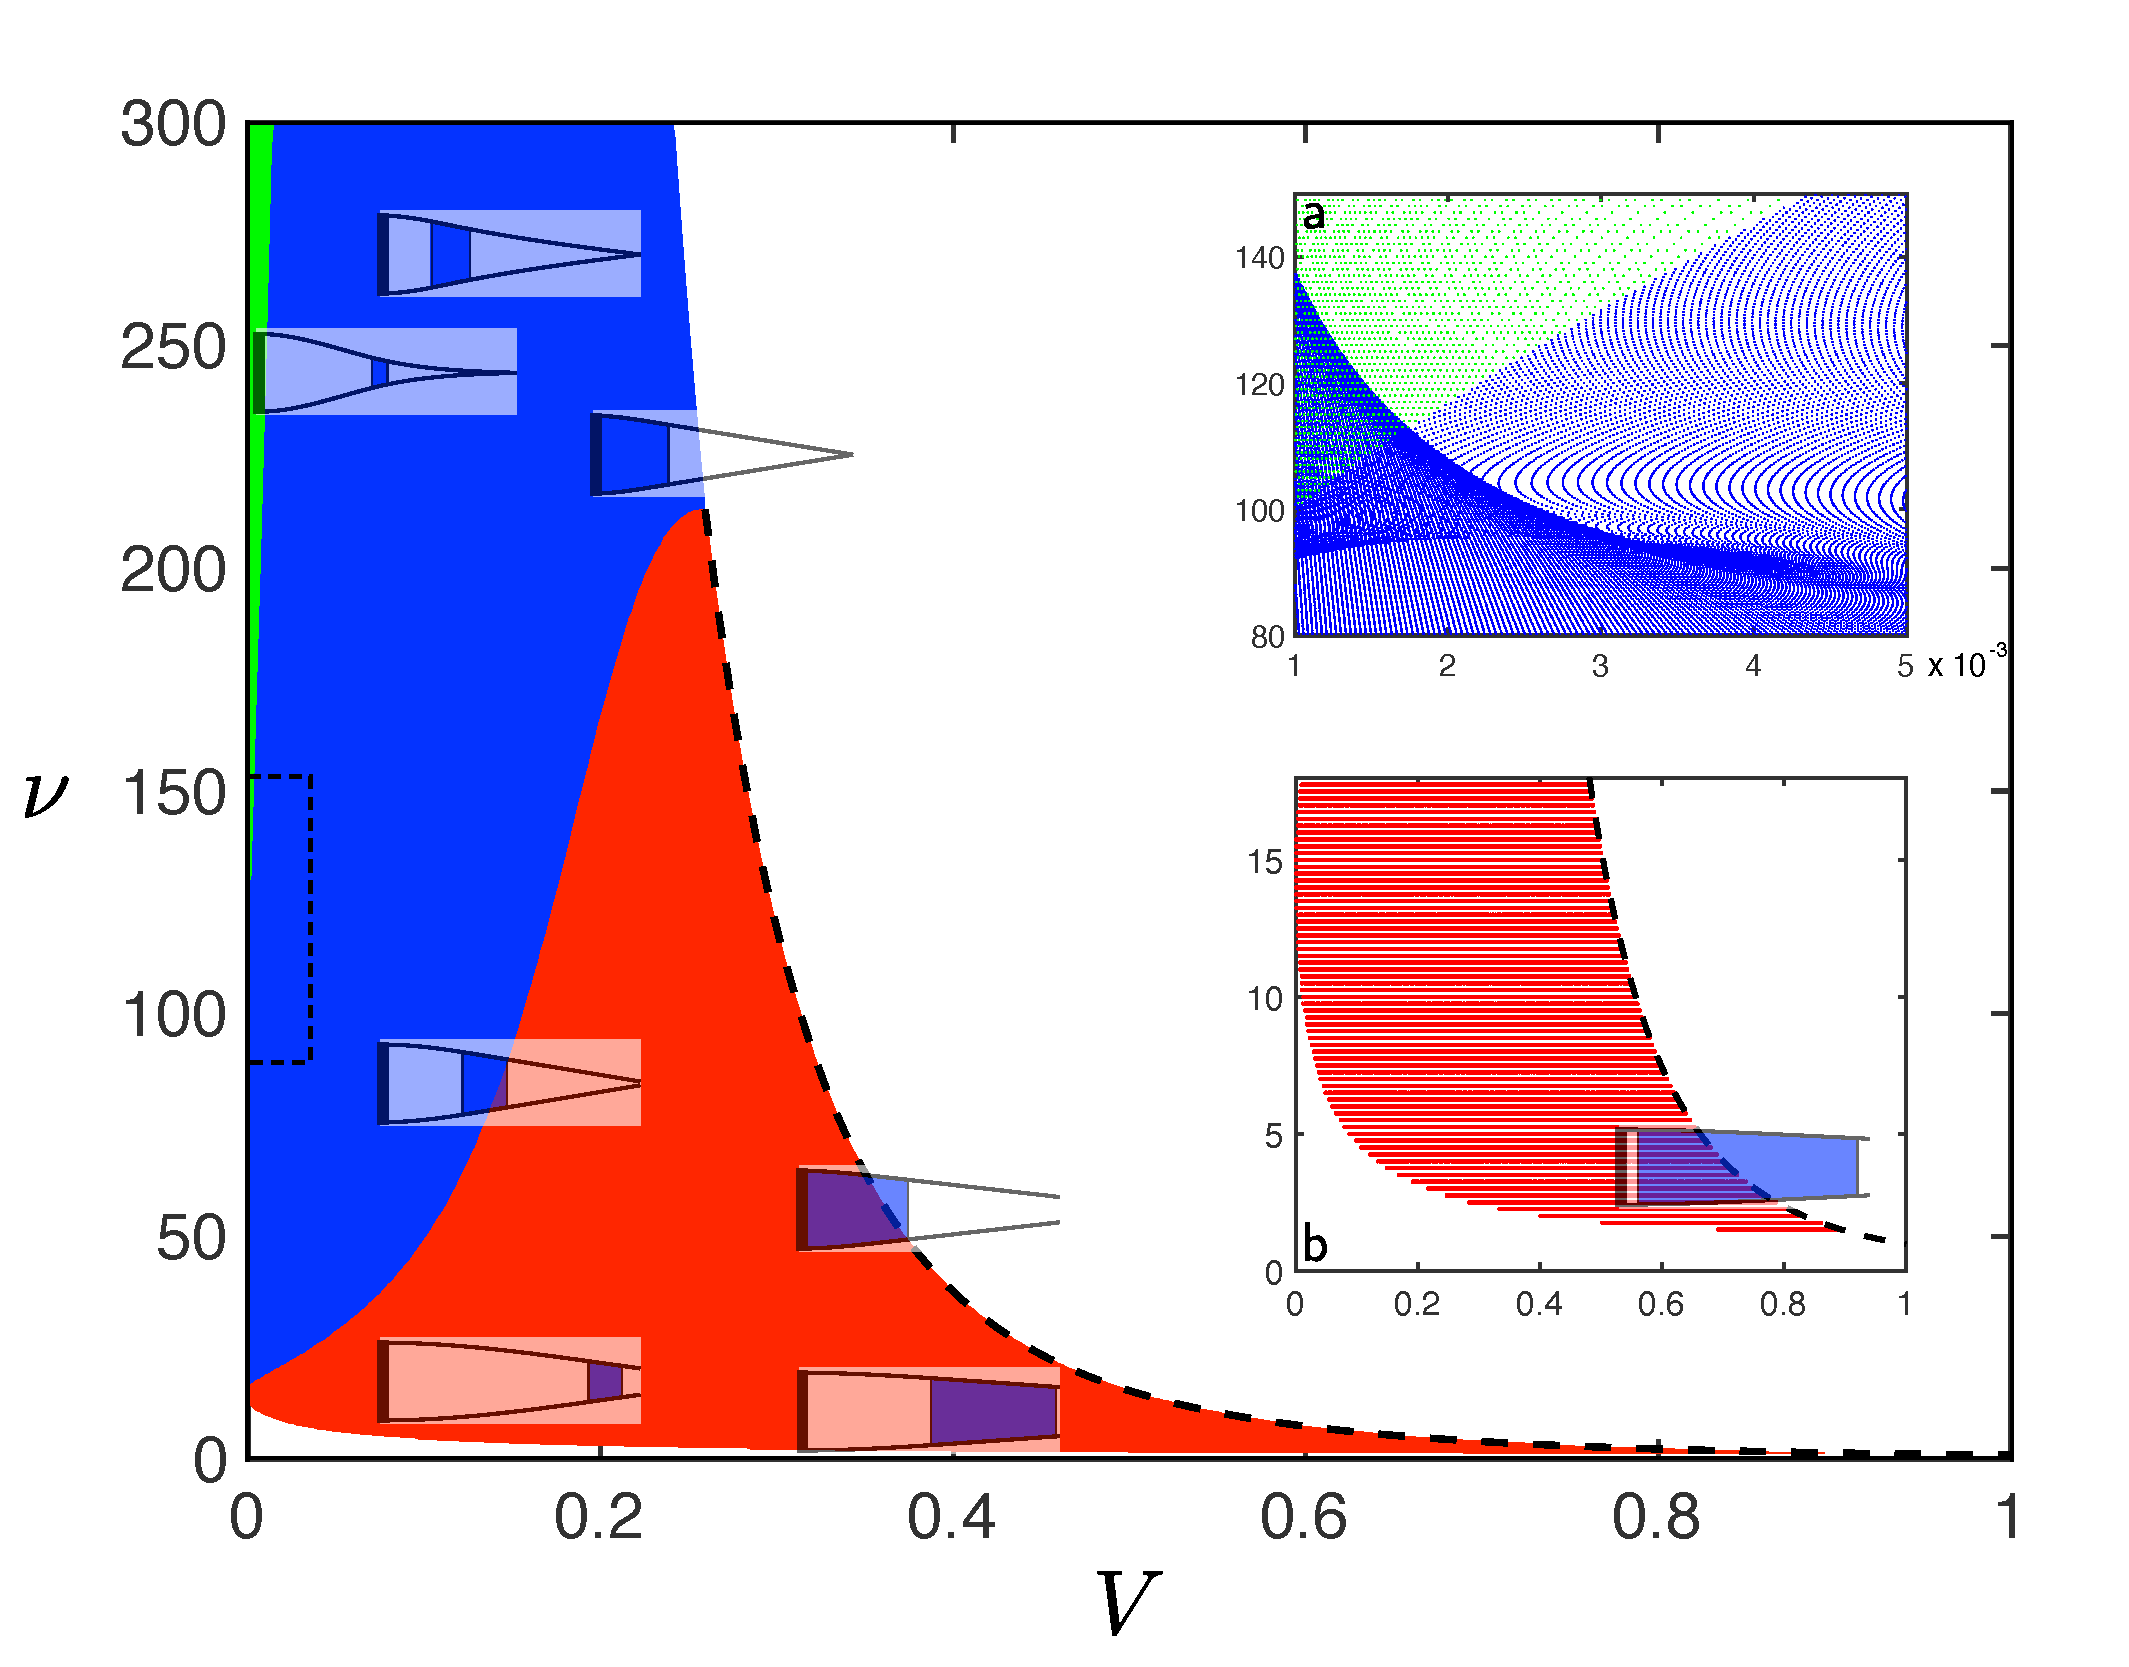
\includegraphics[width = 0.98\textwidth]{detailed_regime_diagram}
\caption{Regime diagram showing regions of $(V, \nu)$ space for which solutions of equations~\eqref{E:Ch4:Hyseresis:Equilibria:Eqs:Beam1}--\eqref{E:Ch4:Hyseresis:Equilibria:Eqs:Volume}  exist with $\hyspare = 0.3$. The schematic diagrams indicate the shape of the configuration close to that region of parameter space. The black dashed curve indicates~\eqref{E:Ch4:Hyseresis:Equilibria:Eqs:analytic_sol_volume}, corresponding to regime I equilibria with $X_- = 0$. Insets are close-ups of the main figure at (a) the dashed box, where multiple solutions exist with the same $(\nu, V)$ values, and (b) the region $0 < \nu < 17$, $0<V<1$. Points corresponding to regimes I, II and III are plotted as red, blue and green points, respectively. }\label{fig:Ch4:Hysteresis:ExampleRegimeDiagram}
\end{figure}

Equilibrium configurations are obtained numerically. Full details can be found in Appendix~\ref{A:Ch4:FindingEquilibria}, but we note that, for convenience, we do not solve the (non-linear) equilibrium equations~\eqref{E:Ch4:Hyseresis:Equilibria:Eqs:Beam1}--\eqref{E:Ch4:Hyseresis:Equilibria:Eqs:Volume} for given $(\nu, V, \hyspare)$ directly; rather we specify one of the meniscus positions (typically $\xlefteq$), and then solve the equations. The volume associated with each equilibrium is then readily calculated using~\eqref{E:Ch4:Hyseresis:Equilibria:Eqs:Volume}. By sweeping over all permissible values of $\xlefteq$, we pick up all possible solutions of~\eqref{E:Ch4:Hyseresis:Equilibria:Eqs:Beam1}--\eqref{E:Ch4:Hyseresis:Equilibria:Eqs:Volume}.

Equation~\eqref{E:Ch4:Hyseresis:Equilibria:Eqs:hyspar_geometry} encodes the fact that equilibria occur when the difference in contact angles $\hyspare$, exactly balances capillary induced wall deflections, whose size depends on the strength of surface tension (via $\nu$), the length over which the force is applied (via $V$) and the position of the droplet (via $\xrighteq$). In Figure~\ref{fig:Ch4:Hysteresis:ExampleRegimeDiagram} we show a regime diagram that indicates the regions of $(V, \nu)$ space in which equilibria exist. By presenting the data in this way, we address the question of how the droplet volume $V$ and bendability $\nu$ interact to create the required channel wall deflection. (Note that this example  with $\hyspare = 0.3$ corresponds to high contact angle asymmetry, but demonstrates the full range of possible behaviour; regime diagrams for smaller values of $\hyspare$ are shown in Figure~\ref{fig:Ch4:Hysteresis:RegimeDiagrams}.)

\begin{figure}[h!]
\centering
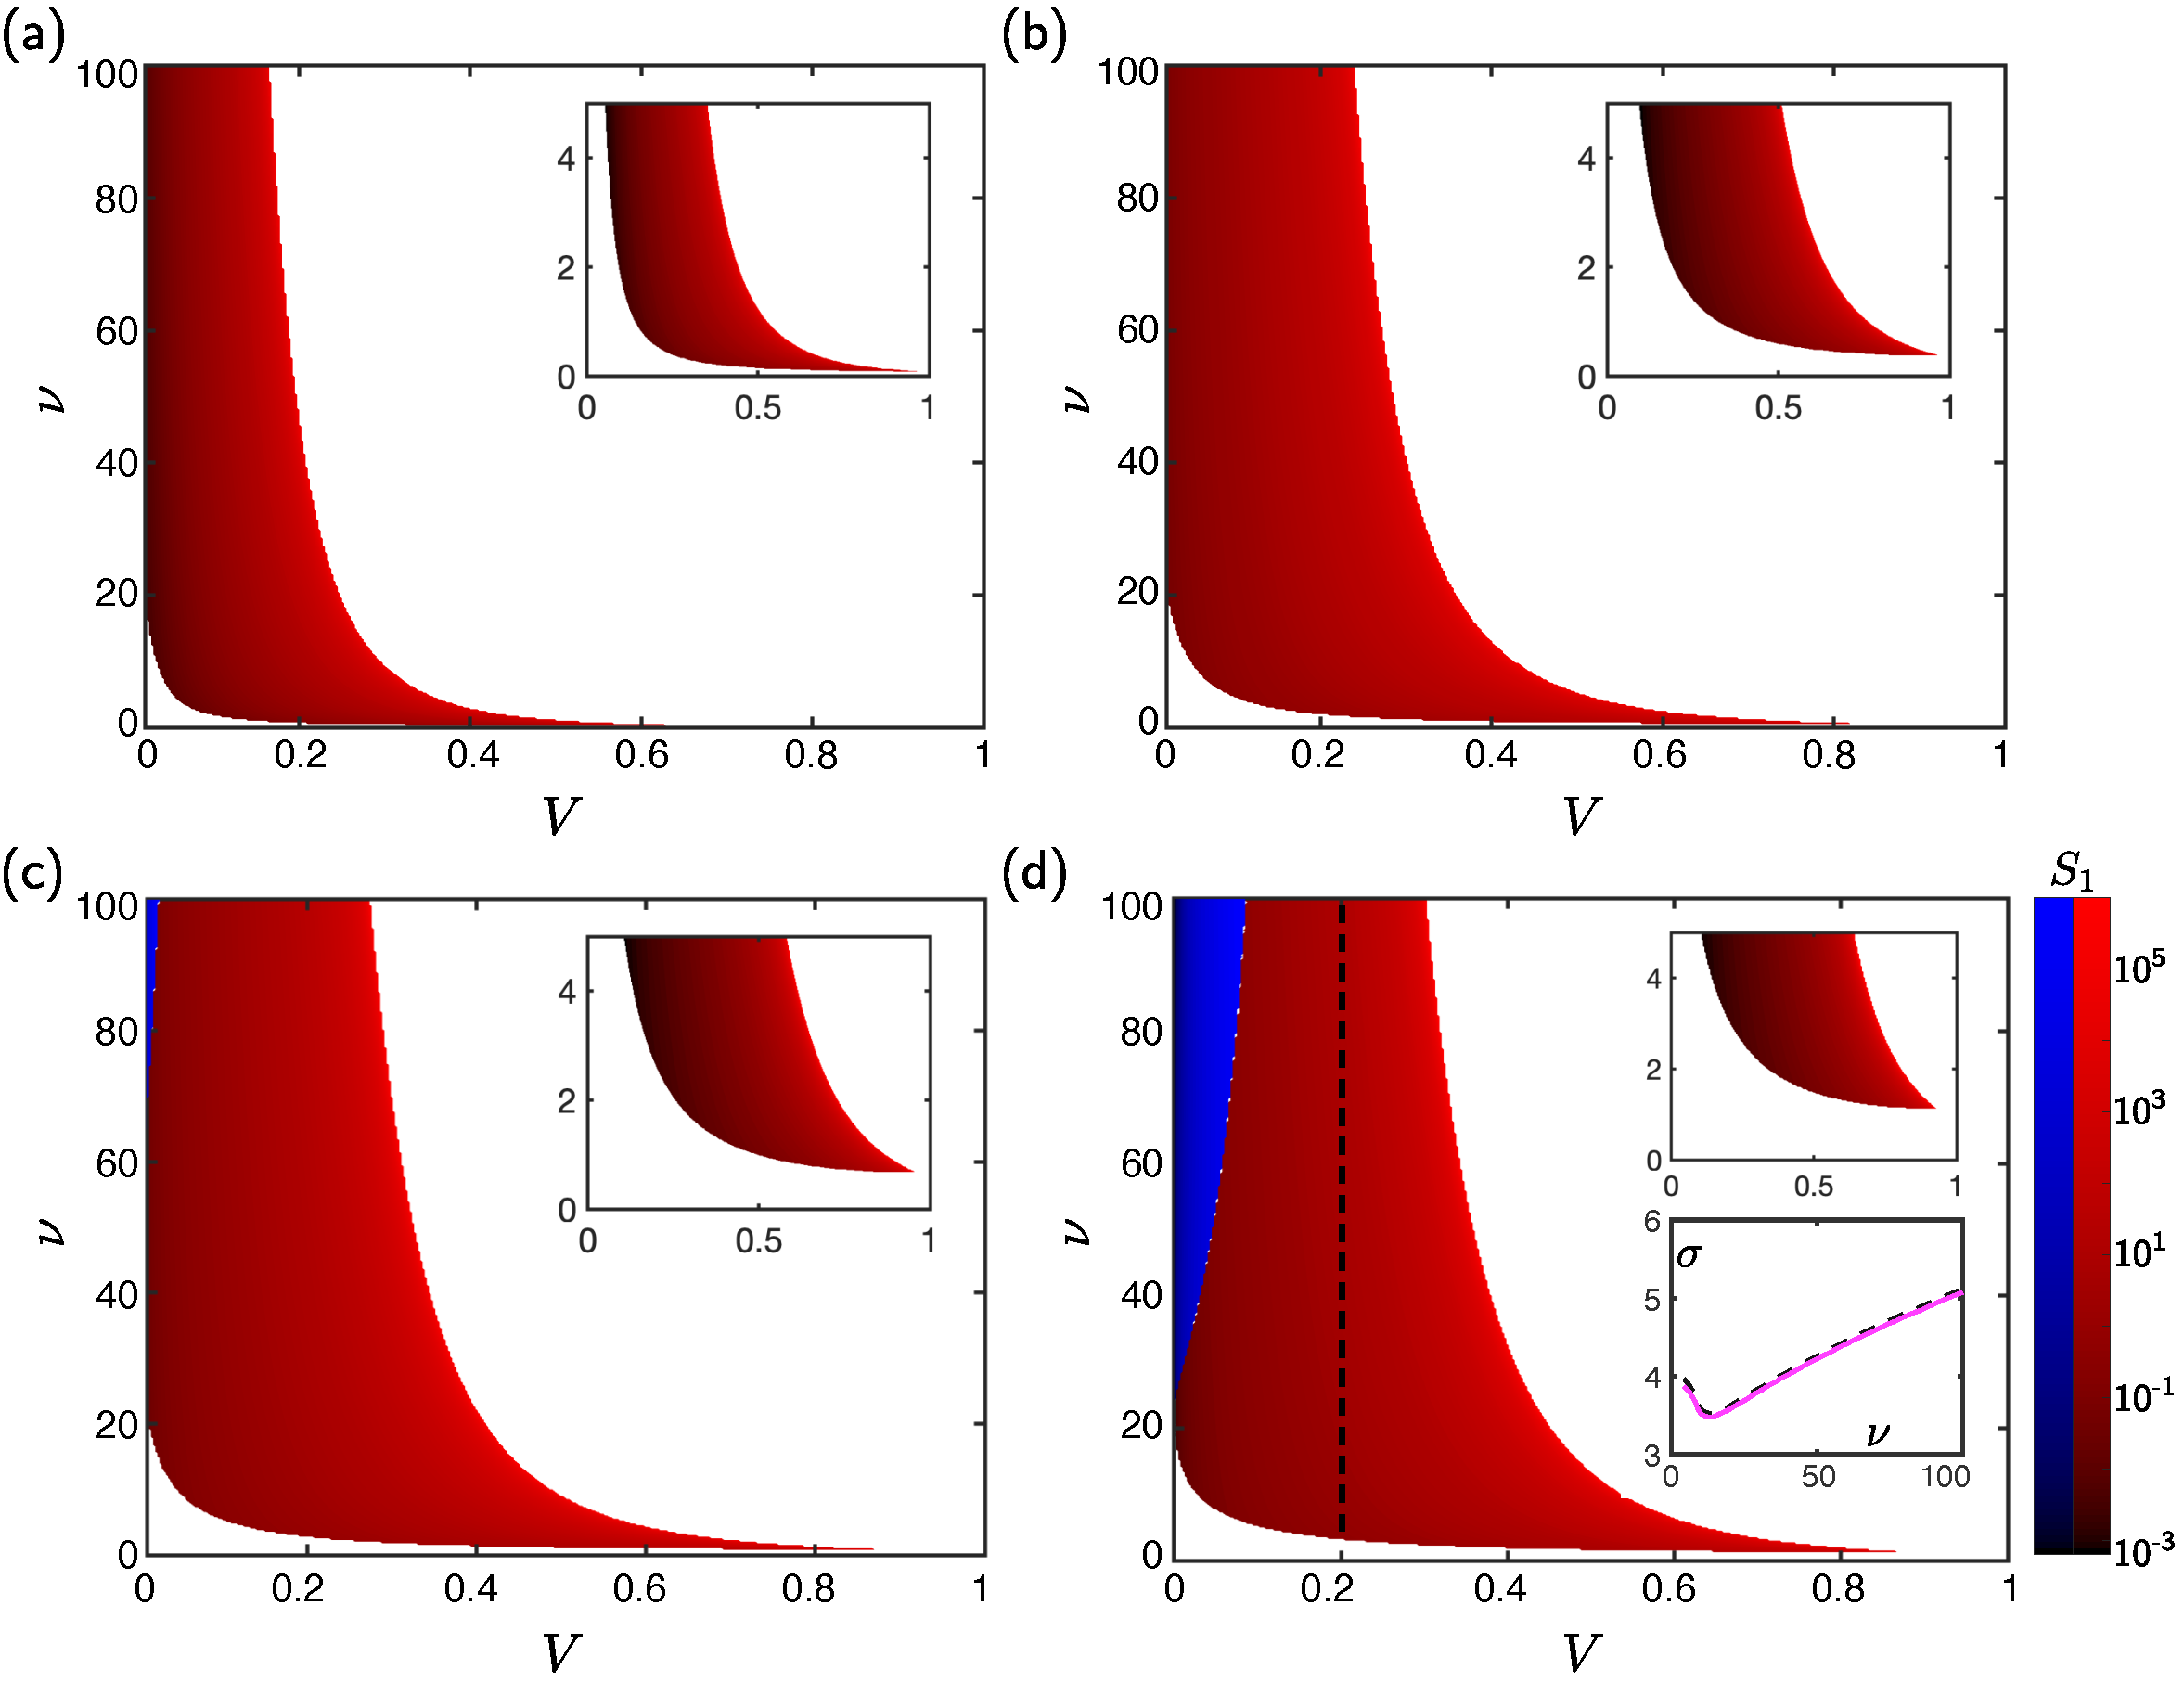
\includegraphics[width = 0.98\textwidth]{example_regime_diagrams}
\caption{Regime diagram showing regions of $(V, \nu)$ space for which solutions of equations~\eqref{E:Ch4:Hyseresis:Equilibria:Eqs:Beam1}--\eqref{E:Ch4:Hyseresis:Equilibria:Eqs:Volume}  exist for (a) $\hyspare = 0.01$, (b) $\hyspare = 0.05$, (c) $\hyspare = 0.1$, and (d) $\hyspare = 0.2$. The inset in each plot is as in the main plot, but zoomed into $0 < \nu < 5$. Red and blue regions indicate regime I  and II equilibria, respectively, and plot shading indicates the value of the constraint $S_1$ (defined in~\eqref{E:Ch4:Hyseresis:Equilibria:Stability:solvability}) according to the colour-bar in (d). The second inset in (d) indicates the growth rates $\sigma$ of perturbations to equilibria with $\hyspare = 0.2, V = 0.2$, as a function of $\nu$ (i.e. along the vertical dashed line in (d)) with the magenta curve corresponding to solutions of the BVP~\eqref{E:Ch4:Hyseresis:Equilibria:Stability:PDE1}--\eqref{E:Ch4:Hyseresis:Equilibria:Stability:kinematic} and the black dashed curve to numerical solutions of the (dynamic) model equations.}\label{fig:Ch4:Hysteresis:RegimeDiagrams}
\end{figure}

We can rationalize the shape of these regime diagrams by considering $\hyspare$ to be a geometric constraint on the capillary induced wall deflections. At small $\nu$ (weak surface tension), the Laplace pressure in the droplet is not able to create enough deflection to satisfy the geometric constraint~\eqref{E:Ch4:Hyseresis:Equilibria:Eqs:hyspar_geometry}, regardless of the droplet's size or position in the channel, and thus no equilibria exist. As $\nu$ increases, equilibria first appear with $\xrighteq = 1$ (see the schematics and inset b in Figure~\ref{fig:Ch4:Hysteresis:ExampleRegimeDiagram}),  since droplets are able to create the largest deflection when they are at the non-clamped end of the channel. This lower boundary of $\nu$ values is decreasing in $V$ (inset b) because larger droplets can generate the same deflection by applying a lower pressure (smaller $\nu$) over a larger area.

As $\nu$ increases (at the same volume $V$), equilibrium configurations have droplets closer to the base, where the higher bendability is countered by pressure being applied over relatively stiffer sections of channel. The channel width at the (currently free) end $x = 1$ is smaller in these equilibria.

Increasing $\nu$ further, regime I equilibria fail to exist when either (i) the channel width at the free end reaches zero, and regime II equilibria appear (blue region in Figure~\ref{fig:Ch4:Hysteresis:ExampleRegimeDiagram}), or, (ii) for larger volume droplets, the lower meniscus reaches the base ($\xlefteq = 0$) -- the droplet can move no further to offset increasing bendability (dashed line in Figure~\ref{fig:Ch4:Hysteresis:ExampleRegimeDiagram}, which corresponds to the analytic result~\eqref{E:Ch4:Hyseresis:Equilibria:Eqs:analytic_sol_volume}--\eqref{E:Ch4:Hyseresis:Equilibria:Eqs:analytic_sol_open_ends}). The boundary between regime II and regime III equilibria behaves in a qualitatively similar way, although it is located at much larger values of $\nu$.


Interestingly, there is a small region  of parameter space where $\nu \gg 1$ and $V \ll 1$ in which multiple equilibria exist (see inset~a in Figure~\ref{fig:Ch4:Hysteresis:ExampleRegimeDiagram}), but elsewhere at most one equilibrium exists. For a general $\hyspare$, the region where multiple equilibria exist is always on the border between regime II and III configurations, and with $V \ll 1$;  because of their small volume, however, these equilibria are considered to be a curiosity (and not physically relevant).

%key points: (i) we have to go to very large nu to get regime II, and regime III is basically non-existant (again can be understood in terms of the geometric constraint), (ii) there is a region of multiple solutions but it's very small (the difference with TV12 is the difference in boundary conditions).

%regime diagrams for different nu, V values.
Regime diagrams for smaller values of the contact angle difference $\hyspar_e$ are shown in Figure~\ref{fig:Ch4:Hysteresis:RegimeDiagrams}. We see that the minimum value of $\nu$ (for a fixed $V$) at which equilibrium configurations exist is smaller for smaller $\hyspar_e$ -- less deflection is needed to satisfy the geometric constraint~\eqref{E:Ch4:Hyseresis:Equilibria:Eqs:hyspar_geometry}, which can therefore be achieved with a lower surface tension. Similarly, the largest value of $\nu$ at which equilibrium configurations exist is also smaller for lower $\hyspare$.  In addition, equilibria in regime II and III are less prevalent; since the border between regime I and II equilibria is well beyond the range of ($\mathcal{O}(1)$) $\nu$ values that are of interest, we shall therefore consider only regime I equilibria for the remainder of this chapter (note that regime III equilibria do exist for $\hyspar_e \leq 0.2$ -- i.e.~in the range of values used in Figure~\ref{fig:Ch4:Hysteresis:RegimeDiagrams} -- but they do not appear on the scale of the plot).

In Figure~\ref{fig:Ch4:Hysteresis:regime_diagrams_xright_and_hyspar_vs_nu} we show two other ways of describing where equilibria exist. Firstly, in Figure~\ref{fig:Ch4:Hysteresis:regime_diagrams_xright_and_hyspar_vs_nu}(a), we plot the value of $\hyspare$ associated with equilibria in $(\xrighteq, \nu)$ space (for the $\mathcal{O}(1)$ values of the bendability $\nu$ that we are interested in). This plot indicates that equilibria in which the droplet is located closer to the free end are associated with a larger $\hyspare$, encoding a larger difference between the channel widths at the menisci, and that this difference is more pronounced for larger $\nu$.

Secondly, in Figure~\ref{fig:Ch4:Hysteresis:regime_diagrams_xright_and_hyspar_vs_nu}(b), we plot the value of $\xrighteq$ associated with equilibria in $(\hyspare, \nu)$ space. In particular, this plot indicates that equilibria do not exist when the contact angle asymmetry $\lambda_e$ is too large (the droplet is not able to create enough deflection to satisfy~\eqref{E:Ch4:Hyseresis:Equilibria:Eqs:hyspar_geometry}, regardless of where it sits in the channel) or too small (the droplet always creates too much deflection, regardless of where it sits in the channel).

\begin{figure}[t]
\centering
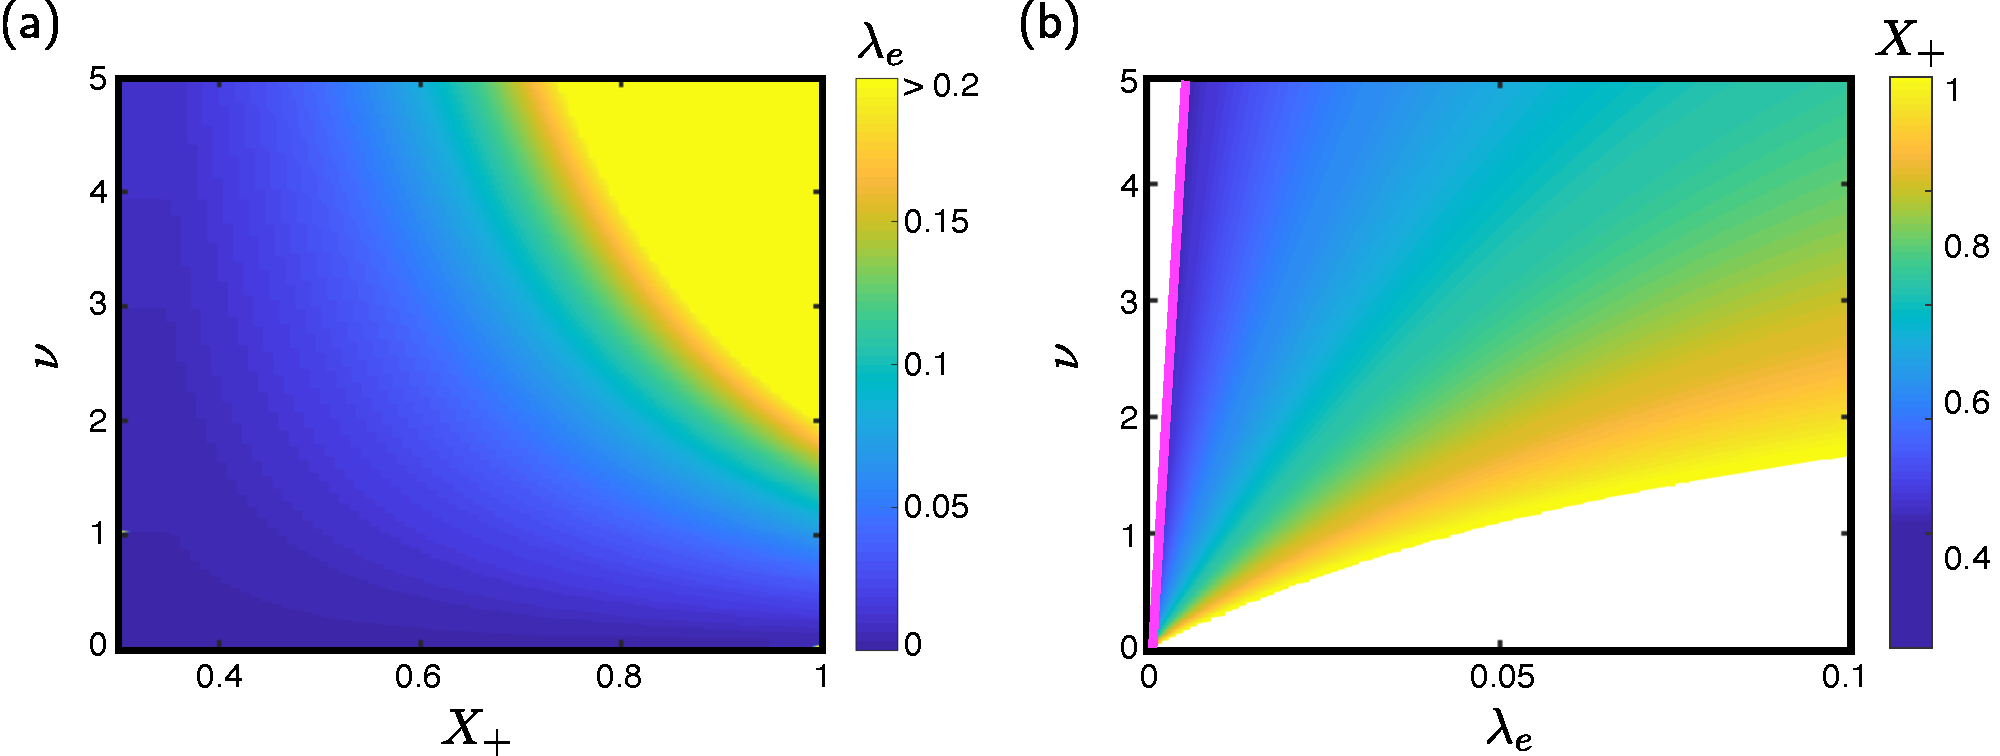
\includegraphics[width = 0.98\textwidth]{xright_and_hyspar_regime_diagram}
\caption{Regime diagrams indicating (a) the value of $\hyspare$ associated with equilibria in $(\xrighteq, \nu)$ space and (b) the value of $\xrighteq$ associated with equilibria in $(\hyspare, \nu)$ space (with $V = 0.3$ in both cases). In (b), no equilibria exist in the white region in the top left and bottom right corners, and the pink line indicates equilibria with $\xlefteq = 0$ (equation~\eqref{E:Ch4:Hyseresis:Equilibria:Eqs:analytic_sol_volume}).}\label{fig:Ch4:Hysteresis:regime_diagrams_xright_and_hyspar_vs_nu}
\end{figure}
\subsubsection{Stability}
We analyze the linear stability of equilibria by letting
\begin{equation}\label{E:Ch4:Hyseresis:Equilibria:Stability:perturbation}
h = h_e(x) + \epsilon e^{\sigma t} h_1(x), \qquad x_{\pm}(t) = \xpmeq +  \xpmeq^1  \epsilon e^{\sigma t} ,
\end{equation}
where $\epsilon \ll 1$ is arbitrary, in the model equations. For simplicity, we assume that the contact angles $\theta_{\pm}$  (and thus $\hyspar= \hyspar_e $), are unchanged by the perturbation (we use the boundary conditions on $h_1$ to reflect the contact angle conditions, see below).

After a standard linearization, the problem for $h_1(x)$ becomes
\begin{align}
0 &= \dd{^4 h_1}{x^4} & & 0 < x < \xlefteq,~\xrighteq < x < 1,\label{E:Ch4:Hyseresis:Equilibria:Stability:PDE1}\\
3|\nu|\sigma h_1 &=\dd{}{x} \left(h_e^3 \dd{^5 h_1}{x^5}\right) & &\xlefteq < x < \xrighteq,\label{E:Ch4:Hyseresis:Equilibria:Stability:PDE2}
\end{align}
with boundary conditions,
\begin{align}
h_1 & = \dd{h_1}{x} = 0 & &\text{at}~x = 0,\\
\dd{^2 h_1}{x^2} &=\dd{^3 h_1}{x^3} = 0 & &\text{at}~x = 1,
\end{align}
continuity conditions,
\begin{align}
\left[h_1 + \xpmeq^1\dd{h_e}{x}\right]_{\xpmeq^-}^{\xpmeq^+} = \left[\dd{h_1}{x} + \xpmeq^1\dd{^2 h_e}{x^2}\right]_{\xpmeq^-}^{\xpmeq^+} &=0, \\ \left[\dd{^2 h_1}{x^2 } +\xpmeq^1 \dd{^3 h_e}{x^3}\right]_{\xpmeq^-}^{\xpmeq^+} = \left[\dd{^3 h_1}{x} +\xpmeq^1 \dd{^4 h_e}{x^4}\right]_{\xpmeq^-}^{\xpmeq^+}  &= 0,
\end{align}
and conservation of volume
\begin{equation}\label{E:Ch4:Hyseresis:Equilibria:Stability:kinematic}
0 = \int_{\xlefteq}^{\xrighteq}h_1 ~\mathrm{d}x - \xrighteq^1 h_e(\xrighteq) + \xlefteq^1 h_e(\xlefteq)
\end{equation}
The final (pressure) boundary conditions on~\eqref{E:Ch4:Hyseresis:Equilibria:Stability:PDE1}--\eqref{E:Ch4:Hyseresis:Equilibria:Stability:PDE2} at $x = \xpmeq$ depend on the pinning conditions. Here we consider two cases. Firstly, mobile conditions,
\begin{align}
\dd{^4h_1}{x^4} &= \frac{\nu(1+ \hyspare)}{h_e^2} \left(\xlefteq^1\dd{h_e}{x} + h_1\right) & &\text{at}~x = \xlefteq,\label{E:Ch4:Hyseresis:Equilibria:Stability:translatingbc1}\\
\dd{^4 h_1}{x^4} &= \frac{\nu}{h_e^2} \left( \xrighteq^1\dd{h_e}{x} + h_1\right)& &\text{at}~x = \xrighteq,\label{E:Ch4:Hyseresis:Equilibria:Stability:translatingbc2}
\end{align}
which are the linearized form of the Laplace pressure boundary conditions~\eqref{E:ch4:Hysteresis:Parametrisation:kbc_and_laplace}b with $\theta_+ = \theta_a$ and $\theta_- = \theta_r$ (i.e. $\hyspare = \hysparmax$) and are thus appropriate for the translating period of the numerical solutions presented in \S\ref{S:Ch4:Hysteresis:Numerics}.

Secondly, we consider a pinned meniscus at $\xlefteq$ and an advancing meniscus at $\xrighteq$, so that
\begin{align}
\dd{^5 h_1}{x^5}&=0 & &\text{at}~x = \xlefteq,\label{E:Ch4:Hyseresis:Equilibria:Stability:pinnedbc1} \\
\dd{^4 h_1}{x^4} &= \frac{\nu}{h_e^2} \left(X_+^1 \dd{h_e}{x} + h_1\right)& &\text{at}~x = \xrighteq,\label{E:Ch4:Hyseresis:Equilibria:Stability:pinnedbc2}
\end{align}
we expect this latter case to be appropriate for the `pinned $\xleft$' period of the numerical solutions of \S\ref{S:Ch4:Hysteresis:Numerics}, where $\hyspar < \hyspar_{\text{max}}$ with $\theta_+ = \theta_a$.

The boundary value problem (BVP) given by~\eqref{E:Ch4:Hyseresis:Equilibria:Stability:PDE1}--\eqref{E:Ch4:Hyseresis:Equilibria:Stability:kinematic} alongside either~\eqref{E:Ch4:Hyseresis:Equilibria:Stability:translatingbc1}--\eqref{E:Ch4:Hyseresis:Equilibria:Stability:translatingbc2} or~\eqref{E:Ch4:Hyseresis:Equilibria:Stability:pinnedbc1}--\eqref{E:Ch4:Hyseresis:Equilibria:Stability:pinnedbc2} may be solved numerically using the \texttt{BVP4c} routine implemented in \textsc{matlab} (for example). This returns the growth rate $\sigma$ as part of the solution. Numerical solutions of the BVP agree well (see inset in Figure~\ref{fig:Ch4:Hysteresis:RegimeDiagrams}(d)) with numerical solutions of the full model equations, in which the growth rate is determined by an exponential fit to the meniscus trajectory at early times.

We do not dwell on solutions on the BVP, however, because we are primarily interested in the stability (the sign of $\sigma$) of equilibria, rather than the time scale of evolution to and from them (the magnitude of $\sigma$). It is instructive to consider instead the marginal stability problem given by~\eqref{E:Ch4:Hyseresis:Equilibria:Stability:PDE1}--\eqref{E:Ch4:Hyseresis:Equilibria:Stability:kinematic} and~\eqref{E:Ch4:Hyseresis:Equilibria:Stability:translatingbc1}--\eqref{E:Ch4:Hyseresis:Equilibria:Stability:translatingbc2} or~\eqref{E:Ch4:Hyseresis:Equilibria:Stability:pinnedbc1}--\eqref{E:Ch4:Hyseresis:Equilibria:Stability:pinnedbc2}  with $\sigma = 0$. In this case~\eqref{E:Ch4:Hyseresis:Equilibria:Stability:PDE2} can be integrated directly to give
\begin{equation}\label{E:Ch4:Hyseresis:Equilibria:Stability:integrate_once}
h_e^3 \dd{^5 h_1}{x^5} = C
\end{equation}
where $C$ is a constant (equal to zero for pinned conditions, from~\eqref{E:Ch4:Hyseresis:Equilibria:Stability:pinnedbc1}). From~\eqref{E:Ch4:Hyseresis:Equilibria:Stability:integrate_once}, we can express $h_1$ in terms of $h_e$, and thus the conservation of volume equations~\eqref{E:Ch4:Hyseresis:Equilibria:Stability:kinematic} can be expressed as a non-linear constraint of the form
\begin{equation}\label{E:Ch4:Hyseresis:Equilibria:Stability:solvability}
S_i(\nu, V, \hyspare) = 0, \qquad i = 1,2.
\end{equation}
Here,  $i = 1$ corresponds to the translating boundary conditions~\eqref{E:Ch4:Hyseresis:Equilibria:Stability:translatingbc1}--\eqref{E:Ch4:Hyseresis:Equilibria:Stability:translatingbc2} and $ i = 2$ to the pinned boundary conditions~\eqref{E:Ch4:Hyseresis:Equilibria:Stability:pinnedbc1}--\eqref{E:Ch4:Hyseresis:Equilibria:Stability:pinnedbc2}.

Solutions to the marginal stability problem exist when~\eqref{E:Ch4:Hyseresis:Equilibria:Stability:solvability} holds. However, we find that $S_i> 0$ over the whole parameter space (the shading in Figure~\ref{fig:Ch4:Hysteresis:RegimeDiagrams} indicates the value of $S_1$), so that for either choice of boundary conditions, the growth rate $\sigma$ does not change sign ($\sigma$ is continuous).

For the translating boundary conditions~\eqref{E:Ch4:Hyseresis:Equilibria:Stability:translatingbc1}--\eqref{E:Ch4:Hyseresis:Equilibria:Stability:translatingbc2}, $\sigma > 0$ \textit{somewhere} in the domain (see inset in Figure~\ref{fig:Ch4:Hysteresis:RegimeDiagrams}(d)), and so $\sigma > 0$. For the pinned boundary conditions~\eqref{E:Ch4:Hyseresis:Equilibria:Stability:pinnedbc1}--\eqref{E:Ch4:Hyseresis:Equilibria:Stability:pinnedbc2}, the same reasoning gives $\sigma <0$ everywhere.

This demonstrates that if the system reaches an equilibrium in which $\xleft$ is pinned, that equilibrium is stable and the droplet remains trapped indefinitely. However, should the droplet reach the translating stage, it will not stop again as any equilibrium it reaches is unstable. (In any case, we do not expect the system to encounter any of these equilibria -- once the droplet has reached the translating stage, the contact angle asymmetry $\hyspar$ cannot increase further, so the pressure difference between the menisci will continue to grow since the channel deflection is enhanced when the droplet is closer to the free end.)

%?????
%need to add a note about our assumption of unchanged contact angles being appropriate for translating conditions, but we expect might  affect equilibria with $\hysparmax - \hyspare \ll 1$ when BC might change as a result of perturbation??


\subsection{Mobile Droplets}
We are now in a position to describe when droplets remain trapped part way along the channel as a result of contact angle hysteresis. We understand that droplets get trapped in stable equilibria  if they remain in the pinned $\xleft$ stage of the motion; this, in turn, is possible, when the maximum contact angle asymmetry, $\hysparmax$, is larger than $\hyspari$, the contact asymmetry required to maintain the pinned state indefinitely.  The crucial point to note is that if an equilibrium exists then the associated contact angle asymmetry $\hyspare(\nu, V, \xrighteq) \approx \hyspari(\nu, V, \xright^0 =\xrighteq)$: for a droplet with given volume $V$ in a channel with given bendability $\nu$, the contact angle asymmetry in equilibrium is approximately that for a pinned droplet with initial condition $\xright^0 = \xrighteq$. (Any difference between $\hyspare$ and $\hyspari$ is a result of the  meniscus motion in the squeezing period, which is brief, making the difference relatively small, see Figure~\ref{fig:Ch4:Hysteresis:ExampleTraces}). As an approximate criterion, therefore, we argue that droplets will be trapped in $\hysparmax \gtrsim \hyspare(\nu, V, \xrighteq = \xright^0)$, and will escape if $\hysparmax \lesssim\hyspare(\nu, V, \xrighteq = \xright^0)$.

With this approximate criterion, the regime diagrams in Figure~\ref{fig:Ch4:Hysteresis:regime_diagrams_xright_and_hyspar_vs_nu} can be re-purposed as maps describing whether droplets will be trapped or not, based on the value of $\hysparmax$ (these regime diagrams are shown again in Figure~\ref{fig:xright_and_hyspar_regime_diagrams} with updated labels to reflect this interpretation of the equilibria). Figure~\ref{fig:xright_and_hyspar_regime_diagrams}(a) therefore (approximately) indicates $\hysparmax^{\textsf{escape}}$, the largest value of $\hysparmax$ at which droplets with initial condition $\xright^0$ are still able to escape: droplets in channels with  $\hysparmax > \hysparmax^{\textsf{escape}}$ will remain trapped, but those in channels with $\hysparmax \leq \hysparmax^{\textsf{escape}}$ will escape. As we see from Figure~\ref{fig:xright_and_hyspar_regime_diagrams}(a) (and as we expected from the numerical solutions presented in \S\ref{S:Ch4:Hysteresis:Numerics}), $\hysparmax^{\text{escape}}$ is increasing in $\xright^0$, so that droplets starting closer to the free end are more likely to escape. We see that, in addition, for a large proportion of the initial droplet positions only a small amount of hysteresis is needed to ensure droplets are trapped ($\hysparmax^{\text{escape}} \ll 1$), again highlighting the sensitivity of our system to contact angle hysteresis.

\begin{figure}[t]
\centering
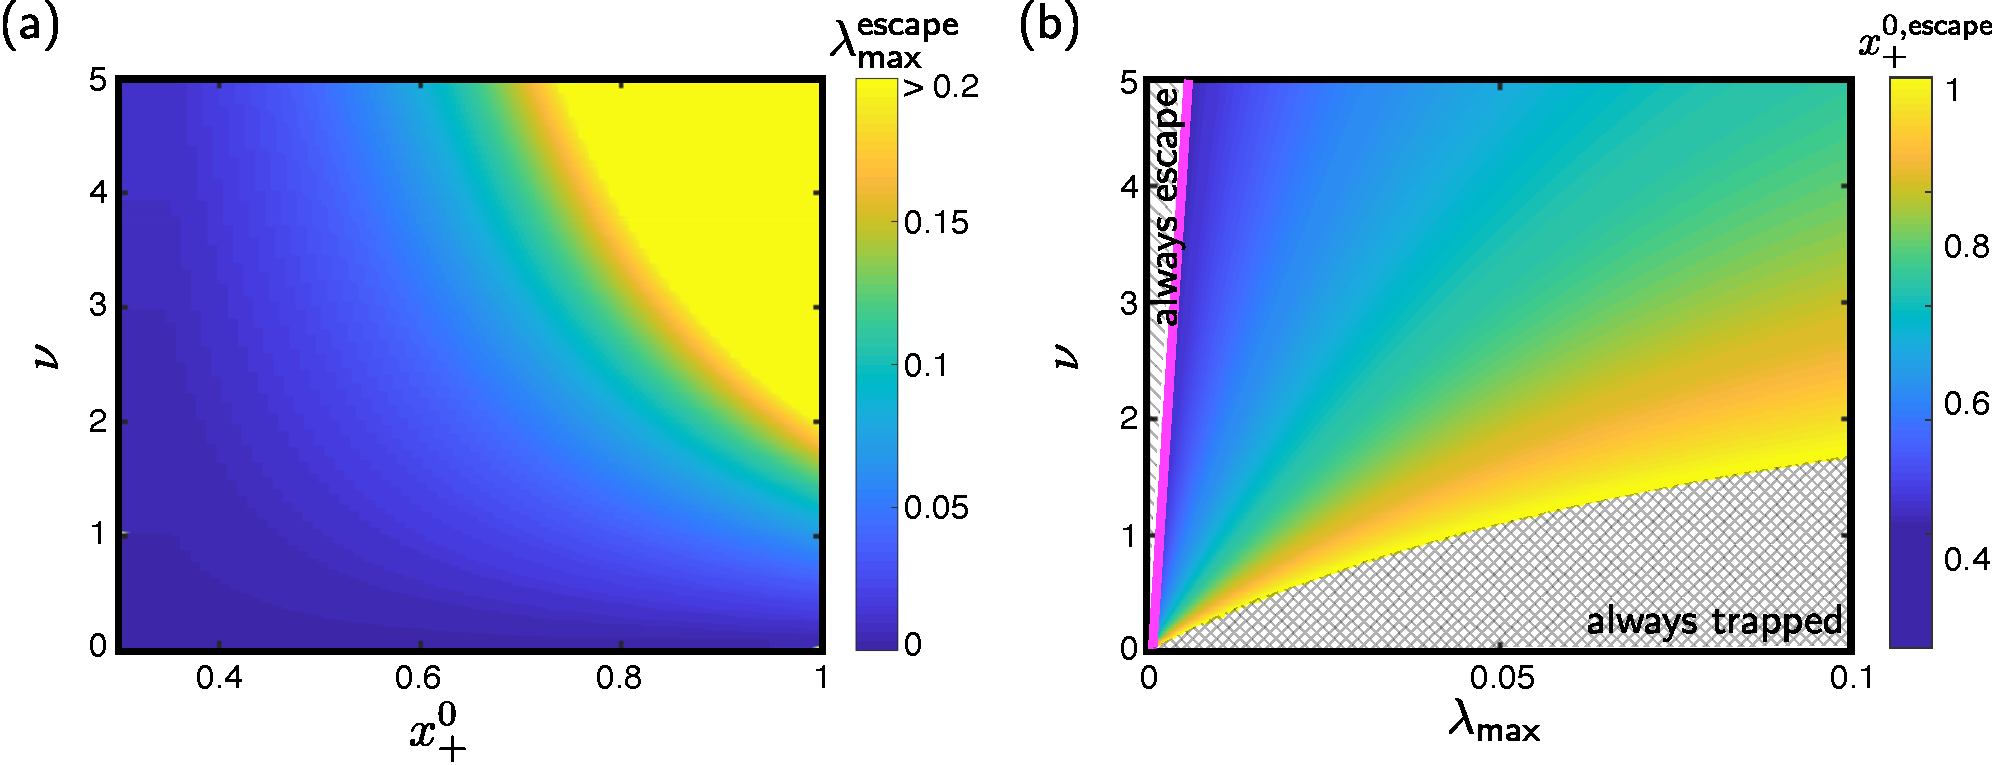
\includegraphics[width = \textwidth]{xright0_and_hysparmax_regime_diagram}
\caption{Predictions from the equilibrium calculation of (a) $\hysparmax^{\text{escape}}$ -- the largest value of $\hysparmax$ at which a droplet with initial position $\xright^0$ is able to escape -- and (b) $\xright^{0,\text{escape}}$ -- how far along the channel a droplet must start in order to escape if the contact angle hysteresis is $\hysparmax$. Both plots correspond to a droplet volume $V = 0.3$. Configurations with $(\hysparmax, \nu)$ that lie in the hatched region (bottom right) will trap droplets of volume $V = 0.3$, regardless of where they start in the channel. Similarly, $V = 0.3$ droplets will escape channels whose $(\hysparmax, \nu)$ lie in the striped region (top left), regardless of where they start in the channel; the pink line indicates the prediction~\eqref{E:Ch4:Hysteresis:MobileDroplets:always_escape_bdry} for the boundary of this `always escape' region.}\label{fig:xright_and_hyspar_regime_diagrams}
\end{figure}

The regime diagram in Figure~\ref{fig:xright_and_hyspar_regime_diagrams}(b)  (in $(\hysparmax, \nu)$ space) can be interpreted as a map showing how far along the channel the droplet must start in order to escape if the contact angle hysteresis if $\hysparmax$; we refer to this `escape position' as $\xright^{0,\textsf{escape}}$.
The equilibrium data for $V = 0.2$ are plotted as a surface in Figure~\ref{fig:Ch4:Hysteresis:escape_surface}; configurations with initial condition $\xright^0 < \xright^{0,\text{escape}}$ (i.e.~beneath this surface) will be trapped, and vice versa -- configurations with initial condition $\xright^0 \geq \xright^{\text{escape}}$ (above this surface) will escape. As expected, with higher hysteresis $\hysparmax$, droplets need to start closer to the free end to escape.

Using the equilibria to predict the $\xright^{0,\text{escape}}$ does not work, however, when such equilibria do not exist. There are two possibilities for configurations whose $(\nu, V, \hysparmax)$ lie in regions of parameter space in which no equilibria exist: if equilibria exist for values of $\hyspar_e$ below $\hysparmax$, then droplets will always be stuck in this channel (the droplet is never able to overcome pinning, since it would need to be located beyond $\xright^0 = 1$ to create enough deflection to do so). Otherwise droplets will always escape (see Figure~\ref{fig:xright_and_hyspar_regime_diagrams}(b) and Figure~\ref{fig:Ch4:Hysteresis:nu_dt_variousV}, which is as in Figure~\ref{fig:xright_and_hyspar_regime_diagrams}(b) for droplet volumes, $V = 0.1$, $0.2$, $0.4$, and $0.5$).

The shape of these `always trapped' regions demonstrate that when surface tension is very weak (small $\nu$) only a small contact angle hysteresis $\hyspar_{\text{max}}$ is needed to ensure that droplets always get stuck, as we might expect. In addition, the contact angle hysteresis needed to ensure that droplets are always trapped reduces for lower volume droplets (that are associated with smaller deflections).

The regions of parameter space in which droplets always escape are only appreciable for larger droplet volumes (note that for $V = 0.1$ and $V = 0.2$ in Figure~\ref{fig:Ch4:Hysteresis:nu_dt_variousV} this region does exist, but is not clearly visible on the scale of the plot). The border of these regions corresponds to equilibria with $\xlefteq = 0$, whose location we expressed analytically in~\eqref{E:Ch4:Hyseresis:Equilibria:Eqs:analytic_sol_volume}--\eqref{E:Ch4:Hyseresis:Equilibria:Eqs:analytic_sol_open_ends}; we therefore predict that droplets will always escape when
\begin{equation}\label{E:Ch4:Hysteresis:MobileDroplets:always_escape_bdry}
\nu > \frac{8}{V^4}\frac{\hyspar_{\text{max}}}{(1+\hyspar_{\text{max}})^2}\left(\frac{3\hyspar_{\text{max}} + 5}{5\hyspar_{\text{max}} + 5}\right)^4.
\end{equation}
The boundary between 'always escaping' and some trapping, given by equality in~\eqref{E:Ch4:Hysteresis:MobileDroplets:always_escape_bdry}, is included as the pink curves in Figure~\ref{fig:xright_and_hyspar_regime_diagrams}(b) and Figure~\ref{fig:Ch4:Hysteresis:nu_dt_variousV}. The sensitive dependence of~\eqref{E:Ch4:Hysteresis:MobileDroplets:always_escape_bdry} on $V$ elucidates why the `always escape' region is not resolved for smaller volume droplets.


\begin{landscape}
\begin{figure}[t]
\centering

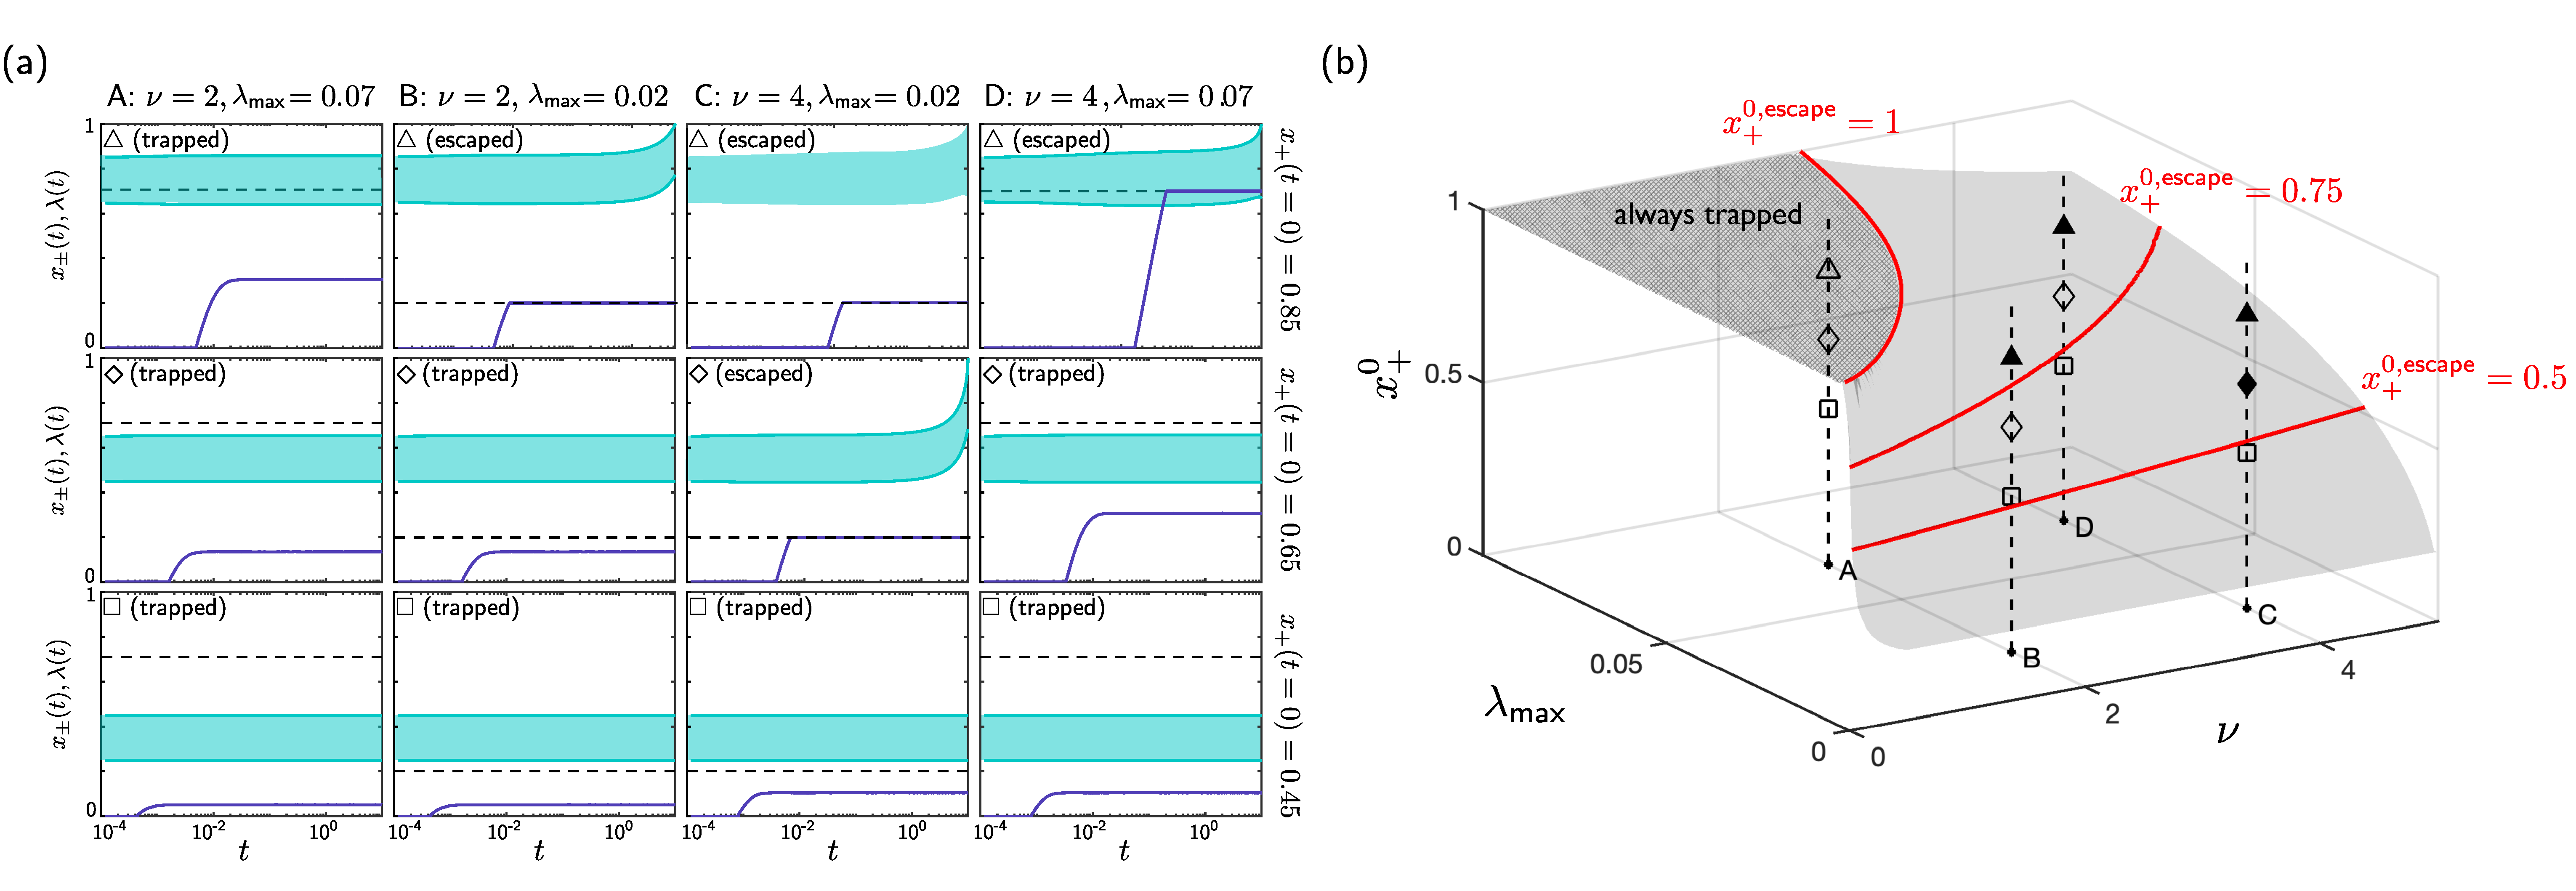
\includegraphics[scale = 0.22]{escape_surface_landscape}
\caption{(a)  Numerically obtained droplet trajectories (the portion of the channel occupied by the droplet is indicated by the green shaded region) as well as the contact angle difference asymmetry $\hyspar$ (purple curve) and contact angle hysteresis $\hyspar_{\text{max}}$ (dashed black line) corresponding to the parameter values at the marked locations (at symbols along dashed lines) in (b). (b) `Escape surface': surface plot of locations of equilibria with $V = 0.2$, interpreted as the boundary between regions of parameters space where droplets will be trapped (below the surface) and regions where droplets will escape (above the surface). Symbols indicate the fate of droplets that start with a particular $\xright^0$: $\triangle$: $\xright^0 = 0.85$, $\diamond$: $\xright^0 = 0.65$, $\square$: $\xright^0 = 0.45$. Filled symbols indicate droplets that escaped ($\hyspar$ reaches $\hysparmax$), open symbols indicate droplets that were trapped ($\hyspar$ does not reach $\hysparmax$).}\label{fig:Ch4:Hysteresis:escape_surface}
\end{figure}
\end{landscape}

\begin{figure}[h!]
\centering
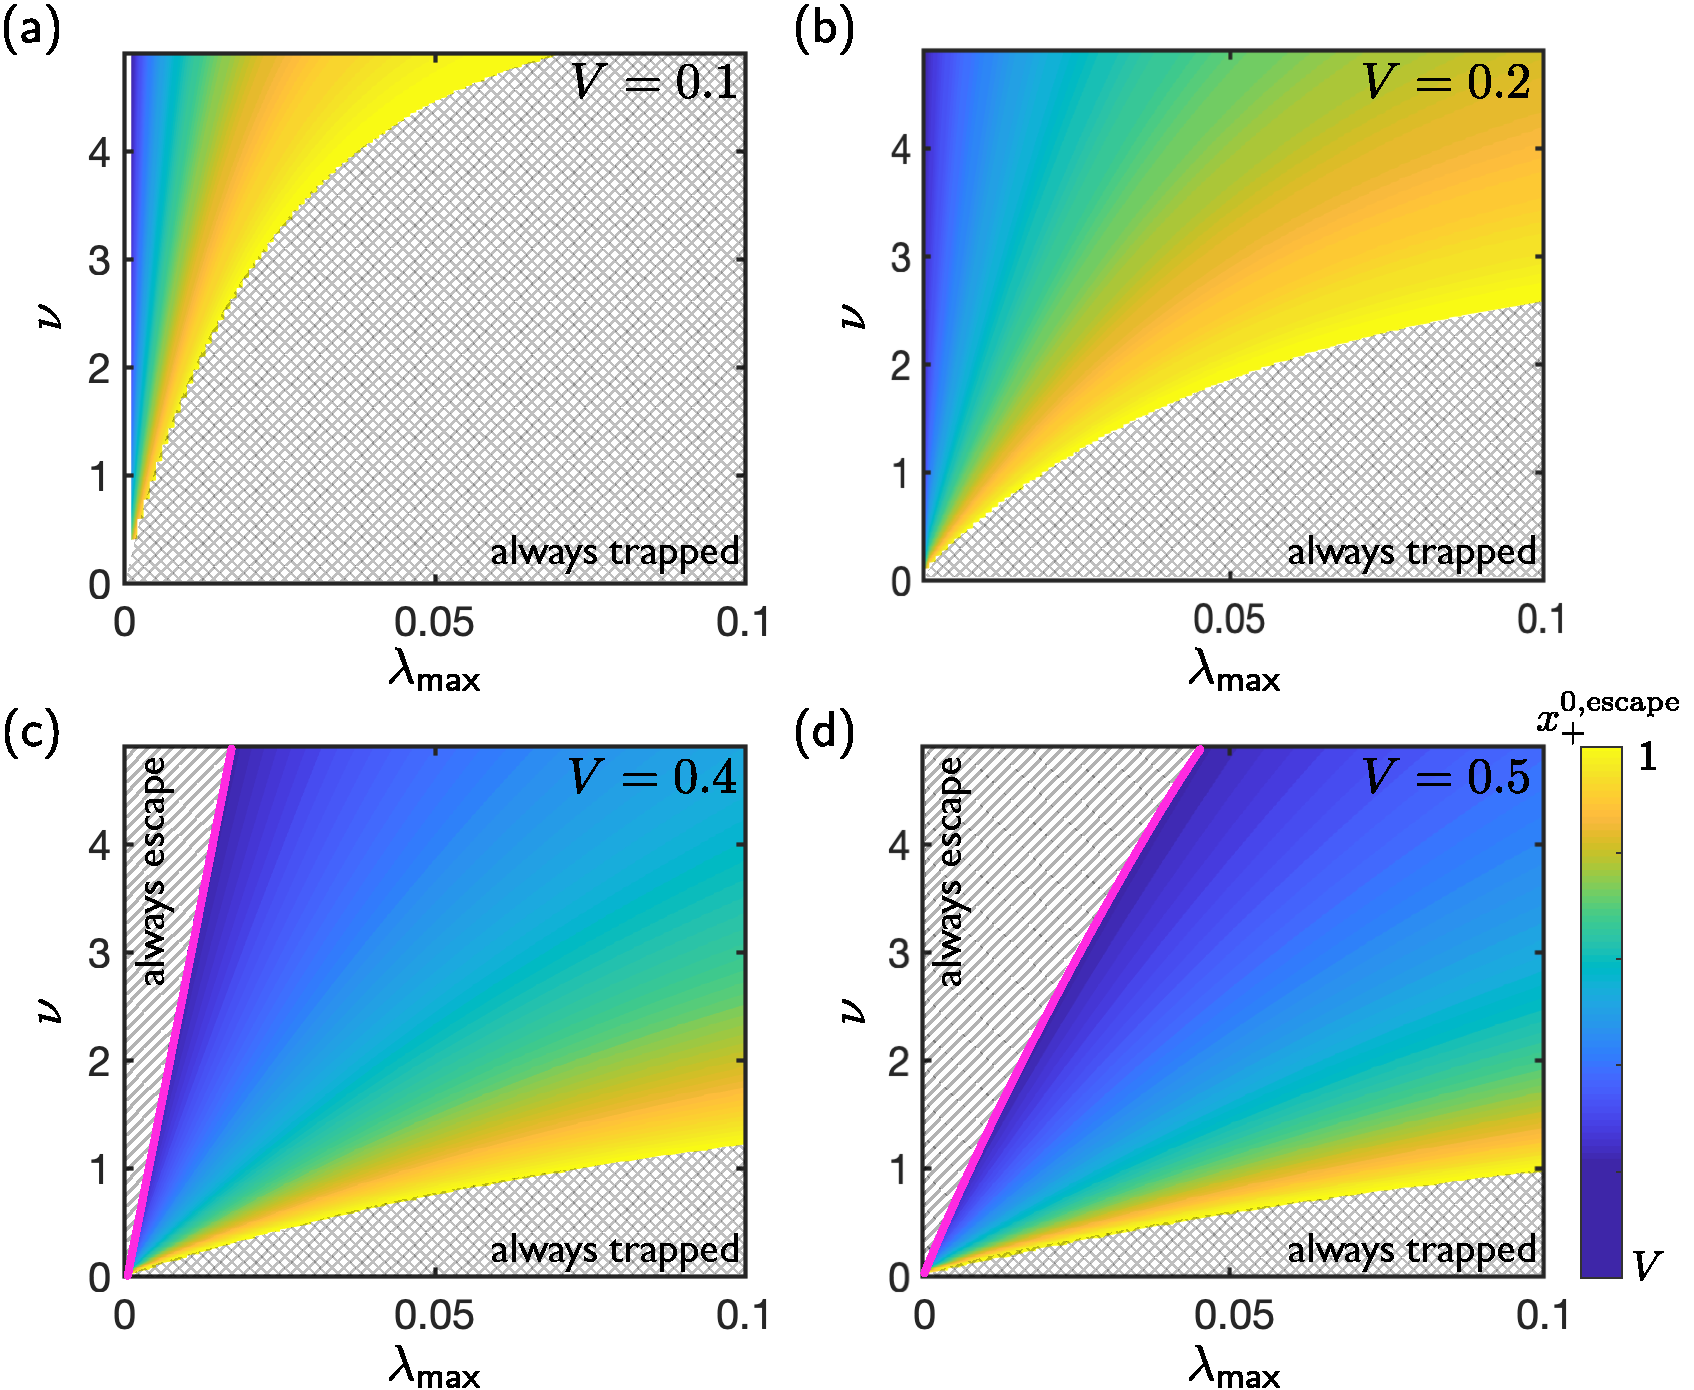
\includegraphics[width = 0.84\textwidth]{nu_dt_regime_diags_diffV}
\caption{Predictions from the equilibrium calculation of  $\xright^{0,\text{escape}}$ -- how far along the channel the droplet must start in order to escape if the contact angle hysteresis is $\hysparmax$ and bendability is $\nu$ (as in Figure~\ref{fig:xright_and_hyspar_regime_diagrams}(b)) for (a) $V = 0.1$, (b) $V = 0.2$, (c) $V = 0.4$, and (d) $V = 0.5$. The colour-bar applies in (d) applies to each plot with the appropriate value of $V$.  Configurations with $(\hysparmax, \nu)$ that lie in the hatched regions (bottom right of each plot) will trap droplets of the corresponding volume, regardless of where they start in the channel. Droplets will escape channels whose $(\hysparmax, \nu)$ lie in the striped region (top left of each plot), regardless of where they start in the channel. The pink line indicates the prediction~\eqref{E:Ch4:Hysteresis:MobileDroplets:always_escape_bdry} for the boundary of `always escape' region (in (a) and (b), this line covers the $y$-axis and is not shown).}\label{fig:Ch4:Hysteresis:nu_dt_variousV}
\end{figure}

%
\subsubsection{Comparison with full numerics}
We compare the results of our equilibrium-based predictions section with numerical results of the full (dynamic) model. To do so, we compute $\xright^{0,\text{escape}}$ numerically using a bisection scheme, with the model equations solved numerically for many different initial conditions. We use $\xright^0 = 0.97$ as a first upper bound to avoid the situation where the `$+$' meniscus is pushed onto the free end $x = 1$ during the initial squeezing; droplets that are trapped even for $\xright^0 = 0.97$ are said to be always be trapped. Similarly, we use $\xright^0 = V + 0.03$ (i.e.~ $\xleft^0 = 0.03$) as the first lower bound; droplets that escape even for $\xright^0 = V + 0.03$ are said to always escape.

The values of $\xright^{0,\text{escape}}$ obtained numerically in this way agree well with the values determined from  equilibrium calculation. This is shown in Figure~\ref{fig:Ch4:Hysteresis:numerics_comparison} where agreement would mean that the colour of the circles in the region where equilibria exist are indistinguishable from the background while the red circles (indicating where droplets never escaped) should be entirely within the empty region towards the right. Note that the numerically determined $\xright^{0,\text{escape}}$ are systematically lower than the equilibrium based predictions (although this is not clearly visible in Figure~\ref{fig:Ch4:Hysteresis:numerics_comparison}), because the equilibrium calculation does not account for the meniscus motion in the squeezing period.

\begin{figure}
\centering
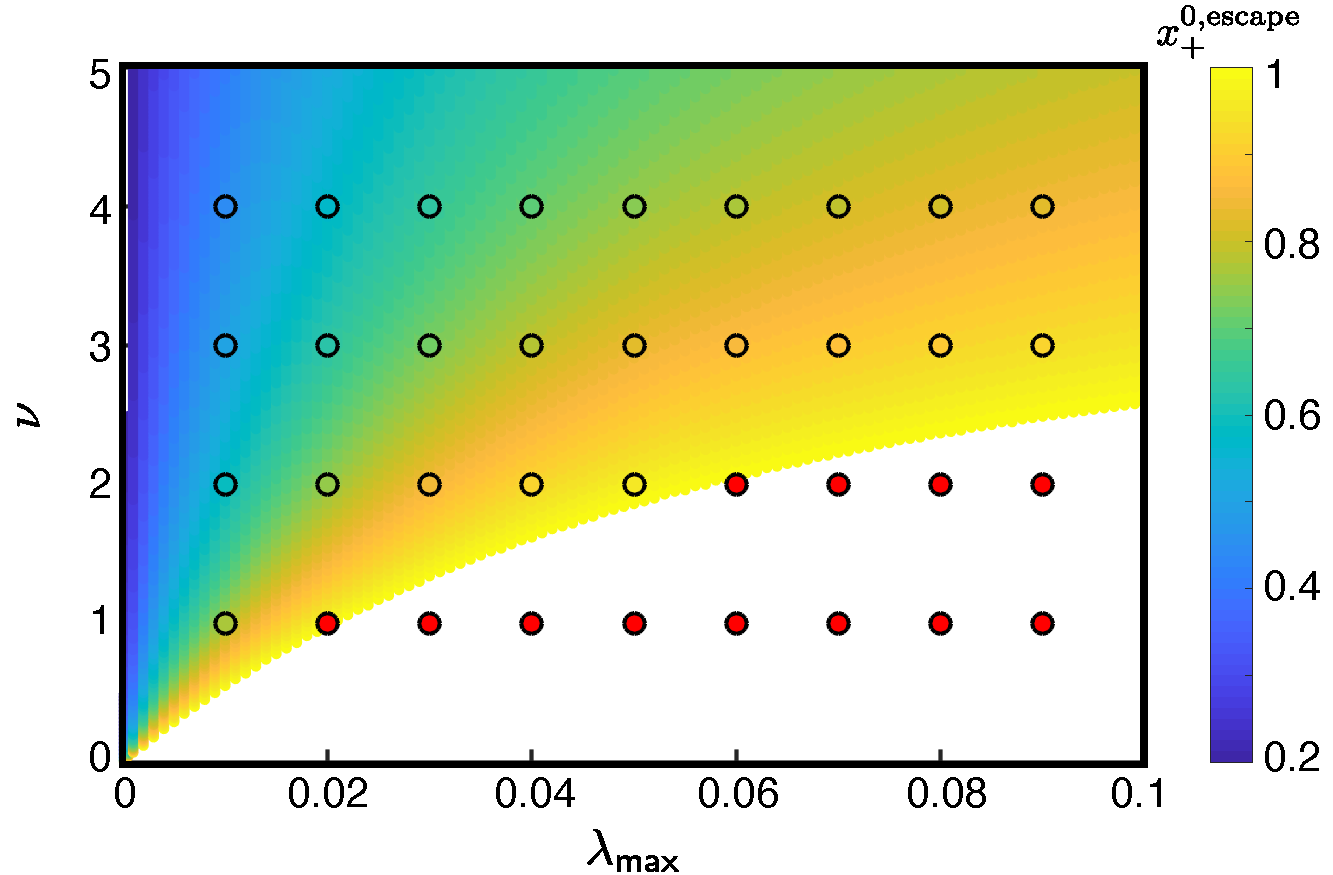
\includegraphics[width = 0.6\textwidth]{numerics_comparison}
\caption{Predictions from the equilibrium calculation (background colour) and numerical solutions of the model equations (circles) for $\xright^{0,\text{escape}}$ with $V = 0.2$. Red markers indicate configurations in which the droplet is always trapped in numerical solutions, regardless of its initial position.}\label{fig:Ch4:Hysteresis:numerics_comparison}
\end{figure}

\subsection{Non-wetting droplets}\label{S:Ch4:Hysteresis:NonWetting}
We conclude this section with a very brief presentation of the corresponding results for non-wetting configurations.

%it's basically the same
The dynamic behaviour of wetting and non-wetting configurations is qualitatively similar: assuming the droplet initially has receding angles at both menisci, an initial squeezing regime is followed by a period in which $\xleft$ is pinned and, possibly, a period in which the droplet translates. Again, droplets can only be trapped during the period for which $\xleft$ is pinned, and not whilst translating.

%here are the always escape and always trapped regions
The mechanism behind droplet trapping in the non-wetting case is exactly the same: in some regions of parameter space, the droplet must begin sufficiently far along the channel if it is to escape. In other regions of parameter space, droplets are trapped regardless of their initial position, and, in others still, they will escape regardless of their initial position; the boundaries between these regions (based on the equilibrium calculation) are indicated in Figure~\ref{fig:Ch4:Hysteresis:trapping_regions_nonwetting} for various droplet volumes $V$. The regions have a qualitatively similar shape to those in the corresponding wetting case (albeit with $\nu \to -\nu$, $\hyspar_{\text{max}} \to -\hyspar_{\text{max}}$); in particular, for small bendability, only a small amount of contact angle hysteresis is required to ensure that droplets are always trapped, and both the always trapped and always escape regions (the latter still given by~\eqref{E:Ch4:Hysteresis:MobileDroplets:always_escape_bdry}) are very sensitive to the value of $V$.

Interestingly, the symmetry $\nu \to -\nu$, $\hyspar_{\text{max}} \to -\hyspar_{\text{max}}$ is not quantitative: Figure~\ref{fig:Ch4:Hysteresis:trapping_regions_nonwetting} shows that the always trapped region is larger, and the always escape region is smaller, for non-wetting configurations than wetting configurations. Without going into detail, the non-linearity in the Laplace pressure boundary condition is responsible for this asymmetry: non-wetting droplets cannot create as large a droplet pressure, and thus deformation, while $\xleft$ is pinned because the meniscus pressure, which scales with $1/h$, does not change as sharply when advancing into an outward tapered channel (increasing $h$) than when advancing into an inward tapered channel (decreasing $h$).

\begin{figure}
\centering
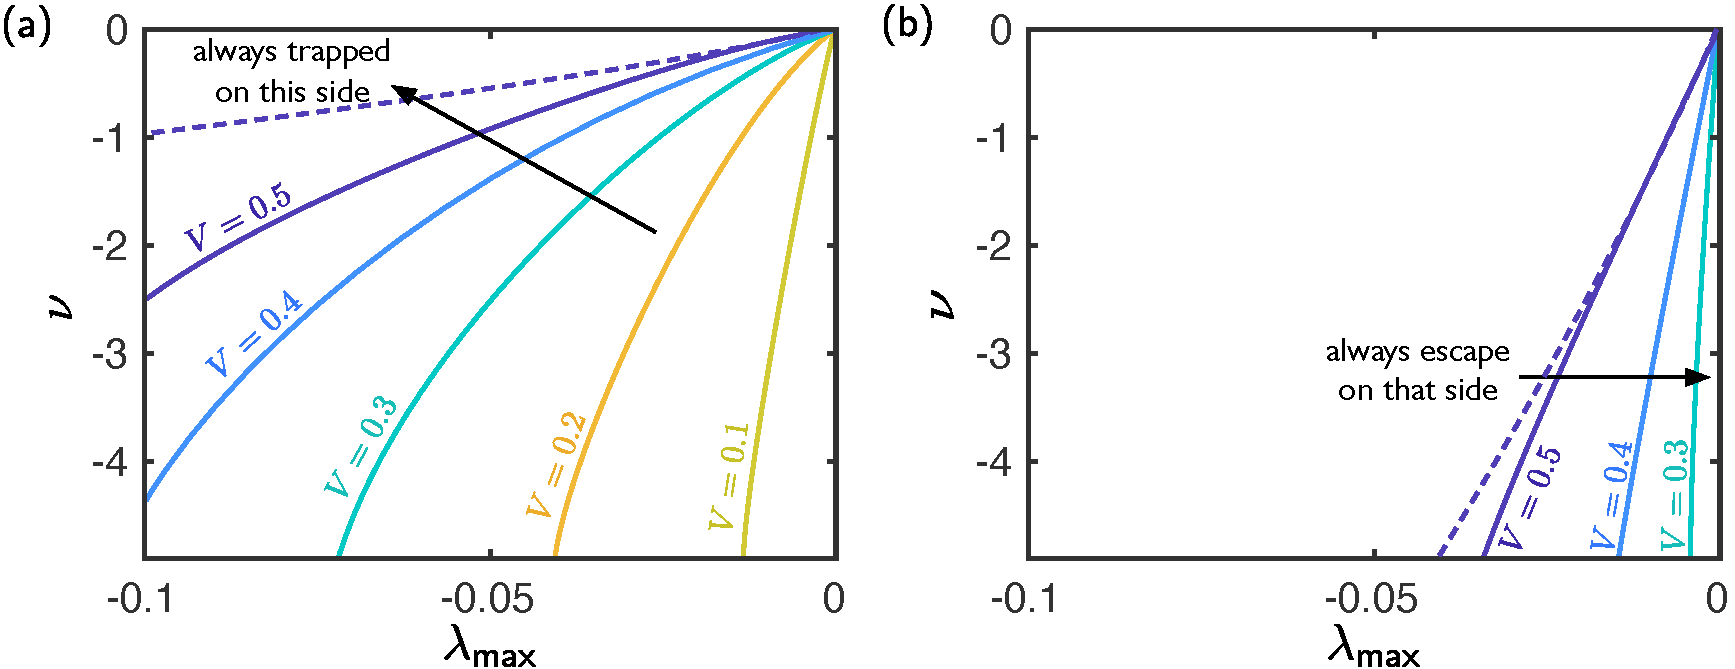
\includegraphics[width = 0.95\textwidth]{non_wetting_escape_and_trapped_regions}
\caption{Boundaries of the regions of $(\hysparmax, \nu)$ space in which (a) droplets are always trapped in the channel, regardless of their initial position, and (b) droplets always escape the channel, regardless of their initial position (based on locations of equilibria). Each boundary corresponds to a different droplet volume. Arrows indicate which side of the boundary droplets are always trapped or always escape, as appropriate. In both plots, the dashed purple curve shows the reflection $\nu \to -\nu, \hysparmax \to -\hysparmax$ of the corresponding boundary for wetting configurations with $V = 0.5$. }\label{fig:Ch4:Hysteresis:trapping_regions_nonwetting}
\end{figure}

\section{Summary}
In this chapter, we have consider two mechanisms through which droplets can be prevented from reaching the free end of the channel. Understanding when droplet motion to the free end of (and thus removal from) the channel is inhibited is important for self-cleaning surfaces that might exploit bendotaxis because trapped droplets might promote the sticky Wenzel state that we are aiming to avoid.

In the first half of the chapter, we considered geometric trapping, which describes the scenario in which the free ends of the channel contact before the droplet reaches the free end. We extended the model developed in Chapter 2 to describe the post-contact behaviour and studied the dynamics of the resulting model through numerical solutions of the model equations. The numerical solutions demonstrated the complex dynamics that result from the competition between the two modes of droplet motion -- squeezing and translating -- as well as from the competition between a diverging meniscus pressure and vanishing channel permeability. In particular, we saw that if the meniscus approaches the end of the channel while the channel walls are simply touching, it appears to reach the end in finite time, with asymptotic behaviour that is faster than previously reported for the analogous rigid case~\citep{Gorce2016Langmuir}. However, if the channel walls touch over an extended portion of their length (as we expect when surface tension is very strong), then the meniscus appears to take an infinite time to reach the cusp.

In the second half of this chapter, we considered trapping by contact angle hysteresis, whose strength is described in our model by the maximum contact angle asymmetry $\hysparmax = \cos \theta_r / \cos \theta_a -1$. Numerical solutions of the model equations confirmed our intuition that when hysteresis is sufficiently strong ($\hysparmax$ sufficiently large), droplets may be trapped in equilibrium part way along the channel. By studying steady solutions of the model equations and assessing their linear stability, we determined that these equilibria are stable and also that droplets will not translate to equilibrium (if droplets start to move appreciably along the channel, they will not be stopped). We identified the importance of the quantity $\hyspari$, the contact angle asymmetry required to hold the droplet in the pinned state (when equilibria are possible). $\hyspari$ gives a simple criterion for whether a droplet will escape: droplets in channels with initial conditions such that the maximum contact angle asymmetry $\hysparmax \leq \hyspari$ will escape, while those with $ \hysparmax > \hyspari$ will not. In reality, $\hyspari$ can only be determined by a full dynamic simulation, but our analysis of equilibria gives  an approximation for $\hyspari$. This approximation allowed us to re-purpose our regime diagrams, that  demonstrate where equilibria exist, to describe whether droplets of given parameters will be trapped or not. In doing so, we identified regions of parameter space in which droplets will always escape and other regions in which droplets are always trapped, regardless of where they start in the channel.  The shape of these regions agreed with our intuition, demonstrating that when the channel bendability is small, only a small amount of contact angle hysteresis is required to trap droplets. In addition, they confirmed that droplets are more likely to be trapped in channels with higher hysteresis, which emphasizes the need to minimize hysteresis in any superhydrophobic surface that might exploit bendotaxis. 


\begin{subappendices}
%\addcontentsline{toc}{section}{Appendices}
\renewcommand{\thesection}{\Alph{section}}
%\appendix

\section{Solving the equations for equilibria}\label{A:Ch4:FindingEquilibria}
In this appendix we describe the method used to find solutions of equations~\eqref{E:Ch4:Hyseresis:Equilibria:Eqs:Beam1}--\eqref{E:Ch4:Hyseresis:Equilibria:Eqs:Volume} describing an equilibrium configuration $h_e(x)$ whose menisci are located at $x = \xpmeq$.

We first `integrate out' the dry regions to give an equivalent problem defined only on the drop region $\xlefteq < x < \xrighteq$ with the effect of the dry regions encoded by effective boundary conditions (as discussed in \S2.2 and \S4.1 for the dynamic problem). In this droplet only problem, the ordinary differential equations, boundary conditions at $x = \xlefteq$ and volume constraint are independent of the nature of any contact at the wall ends (and hence identical for each of the three regimes). We have:
\begin{equation}\label{A:E:Ch4:FindingEquilibria:beam}
\dd{^4 h_e}{x^4} = p_0
\end{equation}
where
\begin{equation}\label{A:E:Ch4:FindingEquilibria:p0}
p_0 =- \frac{\nu}{h_e(\xrighteq)} = - \frac{\nu(\hyspar_e+1)}{h_e(\xlefteq)} \qquad \xlefteq < x< \xrighteq,
\end{equation}
\begin{align}
\left.\dd{^2 h_e}{x^2} - \frac{2}{\xlefteq^2}\left(2\xlefteq \dd{h_e}{x} - 3h_e+3\right)\right|_{x = \xlefteq} &= 0, \label{A:E:Ch4:FindingEquilibria:EffBC_xl1}\\
\left.\dd{^3 h_e}{x^3} - \frac{6}{\xlefteq^3}\left(\xlefteq \dd{h_e}{x} - 2h_e+2\right)\right|_{x = \xlefteq} &= 0.\label{A:E:Ch4:FindingEquilibria:EffBC_xl2}
\end{align}
\begin{equation}\label{A:E:Ch4:FindingEquilibria:Volume}
V = \int_{\xlefteq}^{\xrighteq}h_e(x)~\mathrm{d}x.
\end{equation}
The boundary conditions at $x = \xrighteq$ do depend on the nature of any contact at $x = 1$. For channels in regime I, we have boundary conditions
\begin{equation}\label{A:E:Ch4:FindingEquilibria:EffBC_xu_regimeI}
\dd{^2 h_e}{x^2}  = \dd{^3 h_e}{x^3} =0
\end{equation}
at $x = \xrighteq$. For channels in regime II, we have boundary conditions
\begin{equation}\label{A:E:Ch4:FindingEquilibria:EffBC_xu_regimeII}
(\xrighteq - 1)^3\dd{^3 h_e}{x^3}  - 3\left[(\xrighteq - 1)\dd{h_e}{x} - h_e\right] =
(\xrighteq - 1)\dd{^3 h_e}{x^3}  -\dd{^2 h_e}{x^2} = 0
\end{equation}
at $x = \xrighteq$. For channels in regime III, we have boundary conditions
\begin{equation}\label{A:E:Ch4:FindingEquilibria:EffBC_xu_regimeIII}
\dd{^2 h_e}{x^2} - \frac{6h_e}{(\xrighteq - \xceq)^2} = \dd{^3 h_e}{x^3} - \frac{6h_e}{(\xrighteq - \xceq)^3}=0
\end{equation}
at $x = \xrighteq$, where
\begin{equation}\label{A:E:Ch4:FindingEquilibria:EffBC_xu_regimeIII_xc}
\xrighteq - \xceq - \frac{h_e}{3}\left(\dd{h_e}{x}\right)^{-1}=0.
\end{equation}

For  given $V, \nu$ and $\hyspar_e$, the problem~\eqref{A:E:Ch4:FindingEquilibria:beam}--\eqref{A:E:Ch4:FindingEquilibria:EffBC_xu_regimeIII_xc} for $h_e(x), \xpmeq$ is nonlinear and therefore expensive to solve numerically. It is more convenient to instead specify a meniscus position (typically $\xlefteq$) and solve for $h_e(x)$ and $\xrighteq$ only,  computing the associated volume $V$ a posteriori; with $\xlefteq$ specified the problem~\eqref{A:E:Ch4:FindingEquilibria:beam}--\eqref{A:E:Ch4:FindingEquilibria:EffBC_xu_regimeIII_xc} can be converted into a polynomial in $\xrighteq$ (described below), which is computationally inexpensive to solve.  By sweeping over all permissible values of $\xlefteq$, we pick up all possible equilibria.

In the following sections, we give relevant details of this procedure which differ slightly for channels in regimes I \& II and channels in regime III. We therefore consider these cases separately.

Before we do so, we note that, regardless of the boundary conditions applied at the non-clamped end, the channel shape in the drop region may be expressed as
\begin{equation}\label{A:E:Ch4:FindingEquilibria:Shape}
h_e(x) = \frac{p_0}{24}(x - \xright)^4 + K_3 (x- \xright)^3 + K_2 (x- \xright)^2 + K_1 (x- \xright) + K_0
\end{equation}
where $K_i = K_i(\xrighteq, \xlefteq, p_0),~ i = 1,2,3,4$.
\subsection{Regimes I and II}
The boundary conditions~\eqref{A:E:Ch4:FindingEquilibria:EffBC_xu_regimeI} and~\eqref{A:E:Ch4:FindingEquilibria:EffBC_xu_regimeII} that apply for channels in regime I and II are linear. As a result, the coefficients $K_i, ~i = 1,2,3,4$ in~\eqref{A:E:Ch4:FindingEquilibria:Shape} are linear in the in the equilibrium pressure $p_0$ and multinomials in $\xpmeq$. Using the solution~\eqref{A:E:Ch4:FindingEquilibria:Shape},  the channel displacement at the menisci can be expressed as
\begin{align}
h_e(\xrighteq) &= f_+(\xlefteq, \xrighteq) + p_0 g_+(\xlefteq, \xrighteq), \label{A:E:Ch4:FindingEquilibria:Regime1_and_2:meniscus_disp_1}\\
h_e(\xlefteq) &= f_-(\xlefteq, \xrighteq) + p_0 g_-(\xlefteq, \xrighteq)\label{A:E:Ch4:FindingEquilibria:Regime1_and_2:meniscus_disp_2}
\end{align}
where $f_{\pm}, g_{\pm}$ are known (albeit regime dependent) multinomials.

Inserting~\eqref{A:E:Ch4:FindingEquilibria:Regime1_and_2:meniscus_disp_1}--\eqref{A:E:Ch4:FindingEquilibria:Regime1_and_2:meniscus_disp_2} into the two pressure conditions~\eqref{A:E:Ch4:FindingEquilibria:p0} gives two quadratic equations for the pressure $p_0$:
\begin{align}
p_0 \left[f_+(\xlefteq, \xrighteq) + p_0 g_+(\xlefteq, \xrighteq)\right]  &= -\nu, \label{A:E:Ch4:FindingEquilibria:pressure_quadratic1}\\
 p_0 \left[f_-(\xlefteq, \xrighteq) + p_0 g_-(\xlefteq, \xrighteq)\right]  &= -\nu ( \hyspare+1).\label{A:E:Ch4:FindingEquilibria:pressure_quadratic2}
\end{align}
Eliminating $p_0$ from~\eqref{A:E:Ch4:FindingEquilibria:pressure_quadratic1}--\eqref{A:E:Ch4:FindingEquilibria:pressure_quadratic2} gives a single multinomial whose coefficients depend on parameters $\nu, \hyspare$:
\begin{equation}\label{A:E:Ch4:FindingEquilibria:master_quadratic}
F(\xlefteq, \xrighteq;\nu, \hyspare) = 0.
\end{equation}
Under our assumption that $\xlefteq$ is prescribed, \eqref{A:E:Ch4:FindingEquilibria:master_quadratic} is simply a polynomial equation for $\xrighteq$ (of degree 9 for regime I configurations, and degree 19 for regime II configurations). We solve this polynomial numerically using the \textsc{matlab} routine \texttt{roots}, which computes the eigenvalues of the matrix whose characteristic polynomial is given by~\eqref{A:E:Ch4:FindingEquilibria:master_quadratic}.

Once the equation~\eqref{A:E:Ch4:FindingEquilibria:master_quadratic} has been solved for $\xrighteq$, we keep only those roots that correspond to physically relevant solutions -- i.e. those with $\xlefteq < \xrighteq < 1$ and for which the open end condition~\eqref{E:Ch4:Hyseresis:Equilibria:Eqs:regimeI_constraint} (for channels in regime I), or the repulsive shear and negative slope conditions~\eqref{E:Ch4:Hyseresis:Equilibria:Eqs:regimeII_constraint} (for channels in regime II) are satisfied.

\subsection{Regime III}
The procedure is a little more complicated for configurations in regime III because the boundary conditions~\eqref{A:E:Ch4:FindingEquilibria:EffBC_xu_regimeIII}--\eqref{A:E:Ch4:FindingEquilibria:EffBC_xu_regimeIII_xc} are not linear. As a result, the system of equations for the $K_i$ in~\eqref{A:E:Ch4:FindingEquilibria:Shape} that emerge from  using~\eqref{A:E:Ch4:FindingEquilibria:EffBC_xl1}--\eqref{A:E:Ch4:FindingEquilibria:EffBC_xl2} and~\eqref{A:E:Ch4:FindingEquilibria:EffBC_xu_regimeIII}--\eqref{A:E:Ch4:FindingEquilibria:EffBC_xu_regimeIII_xc} are non-linear in $p_0$. After inserting the result  into the pressure conditions~\eqref{A:E:Ch4:FindingEquilibria:p0} we obtain a system of two quartic equations for the pressure $p_0$.

To obtain solutions of these quartics (for a given $\xlefteq$), we first specify a meniscus position $\xrighteq$ and solve (independently) the resulting quartics in $p_0$. We choose the pair ($\xlefteq, \xrighteq$), and the corresponding pressure $p_0$, to be a candidate equilibrium if any of the roots $p_0$ of the first quartic coincide (to within a tolerance) with any of the roots of the other quartic (we typically choose a tolerance of $0.1$, which is large enough to ensure that we do not miss any solutions but small enough that the search space for the following non-linear solver is not too large). By removing any un-physical roots, and looping over all possible $\xlefteq$, we are left with a set of candidate solutions $\{(\xlefteq^i, \xrighteq^i, p_0^i)\}, ~i =1,\dots, n$.

To find exact solutions of the equilibrium equations, we solve the non-linear equations using \textsc{matlab}'s non-linear equation solving routine \texttt{fsolve}. We provide \texttt{fsolve} with an initial guess at each of the candidate solutions.

Finally, once every possible equilibria has been found in this way, we remove any that violate the sticking condition~\eqref{E:Ch4:Hyseresis:Equilibria:Eqs:regimeIII_constraint}.


\end{subappendices}
